\documentclass[11pt]{article}
\usepackage[turkish,shorthands=:!]{babel}
% Shared preamble for report_en.tex and report_tr.tex
\usepackage[T1]{fontenc}
\usepackage[utf8]{inputenc}
\usepackage{lmodern}
\usepackage{microtype}
\usepackage[a4paper,margin=2.4cm]{geometry}
\usepackage{amsmath,amssymb}
\usepackage{graphicx}
\usepackage{booktabs}
\usepackage{tabularx}
\usepackage{multirow}
\usepackage{xcolor}
\usepackage{float}
\usepackage{caption}
\usepackage{subcaption}
\usepackage{enumitem}
\usepackage{listings}
\usepackage{tikz}
\usetikzlibrary{arrows.meta,positioning,shapes.geometric,fit,calc}
\usepackage{fancyhdr}
\usepackage[hidelinks]{hyperref}

\graphicspath{{../reports/figures/}}
\setlength{\parskip}{0.45em}
\setlength{\parindent}{0pt}
\captionsetup{font=small,labelfont=bf}
\setlist{itemsep=0.15em,topsep=0.3em}

\definecolor{ink}{HTML}{0B0B0B}
\definecolor{ink2}{HTML}{52514E}
\definecolor{accent}{HTML}{2A78D6}
\definecolor{alarm}{HTML}{E34948}
\definecolor{codebg}{HTML}{F6F6F4}
\definecolor{codekw}{HTML}{4A3AA7}
\definecolor{codestr}{HTML}{0F7B55}
\definecolor{codecom}{HTML}{8A8984}

\lstdefinestyle{py}{
  language=Python,
  basicstyle=\ttfamily\footnotesize,
  keywordstyle=\color{codekw}\bfseries,
  stringstyle=\color{codestr},
  commentstyle=\color{codecom}\itshape,
  backgroundcolor=\color{codebg},
  frame=single,
  rulecolor=\color{codebg},
  framesep=4pt,
  numbers=left,
  numberstyle=\tiny\color{codecom},
  numbersep=6pt,
  showstringspaces=false,
  breaklines=true,
  breakatwhitespace=true,
  columns=fullflexible,
  keepspaces=true,
  tabsize=4,
  upquote=true,
  morekeywords={self,None,True,False},
  literate={×}{{$\times$}}1 {≈}{{$\approx$}}1 {→}{{$\to$}}1
}
\lstdefinestyle{plain}{
  basicstyle=\ttfamily\footnotesize,
  backgroundcolor=\color{codebg},
  frame=single,
  rulecolor=\color{codebg},
  framesep=4pt,
  columns=fullflexible,
  keepspaces=true,
  breaklines=true,
  upquote=true
}
\lstset{style=py}

\pagestyle{fancy}
\fancyhf{}
\renewcommand{\headrulewidth}{0.3pt}
\fancyfoot[C]{\thepage}

\newcommand{\code}[1]{\texttt{#1}}
\newcommand{\figw}{\textwidth}

% Pipeline diagram (language-neutral labels are passed as arguments)
\newcommand{\pipeline}[6]{%
\begin{tikzpicture}[
  node distance=0.55cm,
  box/.style={draw=accent!70,fill=accent!6,rounded corners=3pt,align=center,
              minimum height=1.25cm,text width=2.35cm,font=\small},
  arr/.style={-{Stealth[length=2.4mm]},thick,draw=ink2}]
  \node[box] (a) {#1};
  \node[box,right=of a] (b) {#2};
  \node[box,right=of b] (c) {#3};
  \node[box,right=of c] (d) {#4};
  \node[box,right=of d,draw=alarm!80,fill=alarm!6] (e) {#5};
  \draw[arr] (a) -- (b); \draw[arr] (b) -- (c); \draw[arr] (c) -- (d); \draw[arr] (d) -- (e);
  \node[below=0.25cm of c,font=\footnotesize\color{ink2},text width=12cm,align=center] {#6};
\end{tikzpicture}}

\renewcommand{\lstlistingname}{Kod}
\fancyhead[L]{\small\color{ink2}Rulmanlarda Erken Arıza Uyarısı}
\fancyhead[R]{\small\color{ink2}Teknik Rapor}

\title{\textbf{Rulmanlarda Erken Arıza Uyarısı}\\[0.3em]
\large NASA/IMS arızaya kadar çalıştırma (run-to-failure) rulman veri setinde gözetimsiz anomali tespiti ve erken uyarı\\[0.2em]
\normalsize Teknik Rapor}
\author{Ecem Aydemir}
\date{Ekim 2026}

\begin{document}
\maketitle
\thispagestyle{empty}

\begin{abstract}
\noindent
Yuvarlanmalı rulmanlar, döner makinelerdeki arızaların en yaygın kaynaklarından biridir ve
uygulamada arıza etiketleri neredeyse hiçbir zaman bulunmaz. Bu rapor, bir makinenin ömrünün ilk
kısmından \emph{sağlıklı} titreşimin nasıl göründüğünü öğrenen ve bir rulman bu durumdan uzaklaştığında
kararlı (debounce edilmiş) bir alarm üreten, uçtan uca ve yeniden üretilebilir bir erken uyarı sistemini
anlatmaktadır. Sistem, 20\,kHz'de örneklenmiş her bir saniyelik titreşim kaydını fiziksel anlamı olan
18 durum göstergesine (zaman alanı istatistikleri, frekans bandı enerjileri ve rulman arıza
frekanslarındaki zarf spektrumu enerjisi) indirger; dört dedektörü (RMS eşiği temel modeli, Mahalanobis
uzaklığı, Isolation Forest ve LSTM otokodlayıcı) karşılaştırır ve zarf spektrumuna dayalı bir arıza
tipi teşhisi ekler. Geliştirme testinde (IMS test~2) tüm dedektörler, arızalanan rulmanda testin
bitiminden \textbf{yaklaşık 74 saat önce (deney süresinin \%45'i)} kalıcı bir alarm verir ve arızayı
doğru biçimde \textbf{dış bilezik} hasarı olarak teşhis eder. Ayrılmış (held-out) iki testte ise
sonuçlar, uyarı süresi ile yanlış alarm sayısı arasındaki açık bir ödünleşimi ve dürüst bir sınırlamayı
ortaya koyar: makine duruşlarından sonra değişen çalışma koşulları anomali gibi görünmektedir. Çalışma;
tek komutla çalışan bir veri işleme hattı, birim testleri, açıklamalı bir notebook ve etkileşimli bir
Streamlit paneli içeren açık kaynaklı bir Python paketi olarak sunulmaktadır.
\end{abstract}

\tableofcontents
\newpage

%=====================================================================
\section{Giriş}
%=====================================================================

\subsection{Problem}
Kestirimci bakımın amacı bir makineyi arızalanmadan \emph{kısa bir süre önce} onarmaktır: bileşenin
ömrünün büyük kısmını kullanacak kadar geç, müdahaleyi planlayacak kadar erken. Döner makineler için
en zengin bilgi kaynağı titreşimdir ve en sık arızalanan bileşen rulmanlardır. Sensörlü bir makine
sürekli titreşim verisi üretir; ancak bu veri neredeyse hiçbir zaman ``bu rulman şu an bozulmaya
başladı'' diyen etiketlerle gelmez. Arızalar nadir, pahalı ve birbirinden farklıdır; bu nedenle bilinen
arızaları sınıflandırmak üzere eğitilmiş bir model yeni bir makine için genellikle mevcut değildir.

Bu projenin cevapladığı soru şudur:
\begin{quote}
\emph{Yalnızca makinenin sağlıklı olduğu varsayılan bir dönemin verisini kullanarak, bir operatörü bir
rulmanın arızalanmaya başladığı konusunda erken, güvenilir ve az sayıda yanlış alarmla uyarabilir ve
arızanın muhtemel tipini söyleyebilir miyiz?}
\end{quote}

\subsection{Tek paragrafta yaklaşım}
Her titreşim kaydı kompakt bir durum göstergesi vektörüne dönüştürülür. Her deneyin ilk \%25'lik
kısmı sağlıklı kabul edilir ve bir anomali dedektörünü eğitmek için kullanılır; sonraki \%10'luk kısım
alarm eşiğini belirler. Bu noktadan sonra dedektör her yeni kaydı puanlar; son 6 puanın en az 4'ü
eşiği aştığında alarm verilir ve zarf enerjisi en çok artan arıza frekansı muhtemel arıza tipini
belirtir. Sistem üç adet arızaya kadar çalıştırma deneyinde, alarm ile testin bitişi arasındaki saat
sayısı (\emph{uyarı süresi}, lead time) ve makine henüz sağlıklıyken verilen alarm sayısı (\emph{yanlış
alarm}) ile değerlendirilmiştir.

\subsection{Katkılar}
\begin{itemize}
  \item IMS veri seti için sızıntısız (leakage-free), zaman sıralı bir değerlendirme protokolü; tüm üç
        teste ve arızalanan tüm rulmanlara uygulanmıştır. Test~2 geliştirme için kullanılmış, test~1 ve
        test~3 ayrılmış (held-out) olarak tutulmuştur.
  \item Test düzeneğindeki rulmanın gerçek geometrisi için hesaplanmış, arıza frekanslarında zarf
        analizi içeren fiziksel temelli öznitelikler.
  \item Klasik bir temel model, iki klasik makine öğrenmesi dedektörü ve bir derin öğrenme dizi modelinin
        aynı veri bölmeleri, eşikler ve alarm mantığı altında karşılaştırılması.
  \item Operatöre yönelik alarm mantığı (debounce, kalıcılık, ilk alarm veren rulmanla kaynak tespiti
        ve arıza teşhisi) ve bir testi canlı veri akışı gibi yeniden oynatan etkileşimli bir panel.
  \item Yeniden üretilebilir bir yazılım paketi: yapılandırma dosyası, Makefile, birim testleri ve
        depoya eklenmiş öznitelik tabloları (3\,MB). Böylece tüm sonuçlar 6\,GB ham veriyi indirmeden
        yeniden üretilebilir.
\end{itemize}

\subsection{Önceki bir denemeyle ilişkisi}
Bu proje, aynı veri setinde bir LSTM otokodlayıcı eğiten daha önceki bir notebook'un (2025) yeniden ele
alınmasıdır. O çalışmanın incelenmesi, sonuçlarını geçersiz kılan birkaç yöntemsel sorunu ortaya
çıkardı. Bu sorunlar bu veri setinde sık yapılan hatalar olduğu ve Bölüm~\ref{sec:design}'deki tasarım
kararlarını doğrudan yönlendirdiği için burada listelenmiştir:
\begin{enumerate}
  \item \textbf{Model arızalı veriyle eğitilmişti.} Eğitim kümesi deneyin \emph{son} bir milyon
        örneğiydi; yani rulmanın bozulduğu dönem. Aynı veri daha sonra test için de kullanılmıştı.
  \item \textbf{Yanlış rulman izleniyordu.} Test~1'in yalnızca ilk kanalı (rulman~1) kullanılmıştı;
        oysa test~1'de arızalanan rulmanlar 3 ve 4'tür, rulman~1 sağlam kalır.
  \item \textbf{Zaman bilgisi kaybolmuştu.} 2\,156 dosyanın tamamı uç uca eklenip 50 örneklik (2,5\,ms)
        pencerelere bölünmüştü. Zaman ekseni olmadan ``arızadan kaç saat önce uyardı?'' sorusu
        cevaplanamaz.
  \item \textbf{Eğitim ve doğrulama arasında sızıntı.} Üst üste binen pencereler eğitim/doğrulama
        bölmesinden önce karıştırılmıştı; bu nedenle doğrulama kaybı olduğundan iyi görünüyordu.
\end{enumerate}
Önceki çalışmanın temel fikri (``normal''i bir otokodlayıcıyla öğrenip yeniden oluşturma hatasını
anomali puanı olarak kullanmak) korunmuştur; bu rapordaki LSTM otokodlayıcı dedektörü, aynı fikrin
doğru kurulmuş hâlidir.

%=====================================================================
\section{Teorik Arka Plan}
%=====================================================================

\subsection{Yuvarlanmalı rulmanlar ve hasar tipleri}
Bir yuvarlanmalı rulman; mile takılı iç bilezik, gövdeye takılı dış bilezik, yuvarlanma elemanları
(bilye veya makaralar) ve bu elemanları birbirinden ayıran kafesten oluşur. Yorulma, kirlenme veya
yetersiz yağlama bu yüzeylerden birinde lokal bir hasar (oyuk ya da çatlak) oluşturur. Bir yuvarlanma
elemanı hasarın üzerinden her geçtiğinde kısa bir mekanik darbe oluşur. Bu darbeler yalnızca rulman
geometrisine ve mil hızına bağlı bir frekansla tekrarlanır ve rulman ile gövdenin, genellikle kHz
mertebesindeki yapısal rezonanslarını uyarır.

Mil frekansı $f_r$, $n$ adet çapı $d$ olan yuvarlanma elemanı, hatve çapı $D$ ve temas açısı $\phi$
için karakteristik arıza frekansları şunlardır:
\begin{align}
\text{BPFO} &= \frac{n}{2} f_r \left(1 - \frac{d}{D}\cos\phi\right) && \text{(dış bilezik geçiş frekansı)}\\
\text{BPFI} &= \frac{n}{2} f_r \left(1 + \frac{d}{D}\cos\phi\right) && \text{(iç bilezik geçiş frekansı)}\\
\text{BSF}  &= \frac{D}{2d} f_r \left(1 - \left(\frac{d}{D}\cos\phi\right)^2\right) && \text{(yuvarlanma elemanı dönme frekansı)}\\
\text{FTF}  &= \frac{f_r}{2} \left(1 - \frac{d}{D}\cos\phi\right) && \text{(kafes frekansı)}
\end{align}

IMS test düzeneği, sıra başına $n=16$ makaralı, $d = 0{,}331$\,inç, $D = 2{,}815$\,inç ve
$\phi = 15{,}17^\circ$ olan Rexnord ZA-2115 çift sıralı rulmanlar kullanır ve 2000\,dev/dk
($f_r = 33{,}3$\,Hz) hızla döner. Elde edilen frekanslar Tablo~\ref{tab:freqs}'de, kod karşılığı
Kod~\ref{lst:freqs}'de verilmiştir.

\begin{table}[H]
\centering
\caption{ZA-2115 rulmanının 2000\,dev/dk'daki karakteristik arıza frekansları.}
\label{tab:freqs}
\begin{tabular}{lrl}
\toprule
Frekans & Değer [Hz] & İşaret ettiği hasar \\
\midrule
BPFO & 236,4 & dış bilezik \\
BPFI & 296,9 & iç bilezik \\
BSF  & 139,9 & yuvarlanma elemanı \\
FTF  & 14,8  & kafes \\
\bottomrule
\end{tabular}
\end{table}

\begin{lstlisting}[caption={Rulman geometrisinden arıza frekansları (\code{src/bearing\_efw/dataset.py}).},label=lst:freqs]
FS = 20_480  # sampling rate [Hz]
SHAFT_HZ = 2000 / 60.0
N_ROLLERS, ROLLER_D, PITCH_D, CONTACT_ANGLE_DEG = 16, 0.331, 2.815, 15.17

def fault_frequencies(fr: float = SHAFT_HZ) -> dict[str, float]:
    """Characteristic defect frequencies [Hz] for the ZA-2115 bearing."""
    ratio = ROLLER_D / PITCH_D * np.cos(np.deg2rad(CONTACT_ANGLE_DEG))
    return {
        "bpfo": N_ROLLERS / 2 * fr * (1 - ratio),  # outer race
        "bpfi": N_ROLLERS / 2 * fr * (1 + ratio),  # inner race
        "bsf": PITCH_D / (2 * ROLLER_D) * fr * (1 - ratio**2),  # rolling element
        "ftf": fr / 2 * (1 - ratio),  # cage
    }
\end{lstlisting}

\subsection{Titreşim durum göstergeleri}
\paragraph{Zaman alanı istatistikleri.} Ortalaması sıfıra çekilmiş bir $x_1,\dots,x_N$ kaydı için:
\begin{align}
\text{RMS} &= \sqrt{\tfrac{1}{N}\textstyle\sum_i x_i^2}, &
\text{basıklık (kurtosis)} &= \frac{\tfrac{1}{N}\sum_i x_i^4}{\text{RMS}^4}, &
\text{tepe faktörü} &= \frac{\max_i |x_i|}{\text{RMS}}.
\end{align}
RMS toplam titreşim enerjisini ölçer ve endüstriyel standartların çoğunun (ör.\ ISO 10816/20816)
kullandığı göstergedir. Basıklık Gauss gürültüsü için 3'tür ve sinyal keskin darbeler içerdiğinde
büyür; bu nedenle enerji artmadan önce bile erken, lokal hasarlara duyarlıdır. Tepe (crest), biçim
($\text{RMS}/\overline{|x|}$) ve darbe ($\max|x|/\overline{|x|}$) faktörleri benzer darbesellik
ölçüleridir; çarpıklık (skewness) asimetriyi yakalar.

\paragraph{Spektral bant enerjileri.} Güç spektrumunun altı banttaki (0--1, 1--2, 2--4, 4--6, 6--8 ve
8--10,24\,kHz) payı ile spektral ağırlık merkezi, enerjinin \emph{nerede} toplandığını tanımlar.
Gelişen bir hasar enerjiyi yüksek frekanslı rezonanslara doğru kaydırır.

\paragraph{Zarf (envelope) analizi.} Hasar darbeleri kısa sürelidir ve yüksek frekanslı rezonansları
uyarır; bunların \emph{tekrarlanma hızı} (ör.\ BPFO) rezonansın altında gizli kaldığı için ham
spektrumda görünmez. Zarf analizi bu bilgiyi üç adımda geri kazanır \cite{randall2011}:
\begin{enumerate}
  \item sinyal rezonans bölgesinde bant geçiren filtreden geçirilir (burada 2--8\,kHz, 4.\ dereceden
        Butterworth, sıfır faz),
  \item analitik sinyalin (Hilbert dönüşümü) genliği alınır; bu, genlik modülasyonlu rezonansın
        zarfıdır,
  \item zarfın spektrumu hesaplanır; lokal bir hasar, karakteristik frekansında ve harmoniklerinde
        tepe üretir.
\end{enumerate}
Burada kullanılan öznitelik, zarf spektrumu enerjisinin (5--1000\,Hz) BPFO, BPFI ve BSF'nin ilk üç
harmoniğinin $\pm3$\,Hz çevresine düşen payıdır.

\subsection{Gözetimsiz anomali tespiti}
Arıza etiketi kullanılmadığı için tüm dedektörler \emph{tek sınıflı} (one-class) veya \emph{yenilik}
(novelty) dedektörleridir: yalnızca sağlıklı veriyle eğitilirler ve yeni bir gözlem sağlıklı veriye
ne kadar az benziyorsa o kadar büyük bir puan üretirler.

\paragraph{Mahalanobis uzaklığı.} Sağlıklı öznitelik vektörlerinin ortalaması $\boldsymbol\mu$ ve
kovaryansı $\boldsymbol\Sigma$ ile
\begin{equation}
d_M(\mathbf{x}) = \sqrt{(\mathbf{x}-\boldsymbol\mu)^\top \boldsymbol\Sigma^{-1}(\mathbf{x}-\boldsymbol\mu)}.
\end{equation}
Bu ölçü öznitelikler arasındaki korelasyonları (ör.\ RMS ve tepe değeri) hesaba katar. Pek çok
öznitelik birbiriyle ilişkili ve eğitim kümesi küçük olduğundan $\boldsymbol\Sigma$, örnek kovaryansı
ölçeklenmiş birim matrise doğru çekerek iyi koşullu tutan Ledoit--Wolf büzülme (shrinkage) yöntemiyle
kestirilir \cite{ledoit2004}.

\paragraph{Isolation Forest.} Gözlemleri rastgele bölmelerle yalıtan rastgele ağaçlardan oluşan bir
topluluktur \cite{liu2008}. Anomaliler az sayıda ve farklı oldukları için daha az bölmeyle yalıtılır;
puan ortalama yol uzunluğundan türetilir.

\paragraph{LSTM otokodlayıcı.} Otokodlayıcı girdisini düşük boyutlu bir gizli koda sıkıştırır ve
yeniden oluşturur. Yalnızca sağlıklı veriyle eğitildiğinde sağlıklı girdileri iyi, tanımadığı girdileri
kötü yeniden oluşturur; bu nedenle $W$ kayıt ve $p$ öznitelikten oluşan bir pencere üzerindeki
yeniden oluşturma hatası
\begin{equation}
e_t = \frac{1}{W\,p}\sum_{k=0}^{W-1}\sum_{j=1}^{p}\left(x_{t-k,j}-\hat{x}_{t-k,j}\right)^2
\end{equation}
bir anomali puanıdır \cite{malhotra2016}. Uzun kısa süreli bellek (LSTM) katmanları
\cite{hochreiter1997} modelin pencere içindeki zamansal değişimi kullanmasını sağlar.

\paragraph{RMS eşiği.} Her bakım mühendisinin ilk deneyeceği temel yöntem: toplam titreşim seviyesi
sağlıklı aralığının üstüne çıktığında alarm. Daha karmaşık bir yöntemin karmaşıklığına değmesi için
bunu geçmesi gerekir.

%=====================================================================
\section{Veri Seti}
%=====================================================================

IMS rulman veri seti \cite{lee2007,qiu2006}, Cincinnati Üniversitesi'ndeki NSF I/UCR Akıllı Bakım
Sistemleri Merkezi (Center for Intelligent Maintenance Systems) tarafından üretilmiş ve NASA Prognostik
Mükemmeliyet Merkezi (PCoE) tarafından dağıtılmaktadır. Bir AC motorla sabit 2000\,dev/dk'da döndürülen
tek bir mil üzerinde dört rulman bulunur ve bir yay mekanizmasıyla 6000\,lb radyal yük uygulanır. Rulman
gövdelerindeki ivmeölçerler (PCB 353B33) bir NI DAQCard-6062E ile 20\,kHz'de örneklenir. Her 10 dakikada
bir (test~1'in başında 5 dakikada bir) kanal başına 20\,480 örnekten oluşan bir saniyelik bir kayıt, adı
zaman damgası olan bir metin dosyasına yazılır. Her test bir rulman arızalanana kadar sürdürülmüştür.

\begin{table}[H]
\centering
\caption{Üç arızaya kadar çalıştırma testi. Süre, ölü kayıtlar çıkarıldıktan sonra ölçülmüştür.}
\label{tab:tests}
\begin{tabularx}{\textwidth}{lrlrX}
\toprule
Test & Kayıt & Kanal & Süre [sa] & Test sonundaki arıza \\
\midrule
test1 & 2\,156 & 8 (rulman başına x, y) & 827,6  & rulman 3 iç bilezik, rulman 4 yuvarlanma elemanı \\
test2 & 984    & 4                      & 163,5  & rulman 1 dış bilezik \\
test3 & 6\,324 & 4                      & 1\,073,1 & rulman 3 dış bilezik \\
\bottomrule
\end{tabularx}
\end{table}

\paragraph{Veriyle çalışırken keşfedilen pratik ayrıntılar.}
\begin{itemize}
  \item Arşiv, içinde bir 7-Zip dosyası, onun içinde de üç RAR dosyası bulunan bir ZIP'tir (yaklaşık
        1\,GB indirme, açıldığında 6,2\,GB, 9\,464 kayıt dosyası).
  \item \code{3rd\_test.rar} dosyası \code{4th\_test/txt} adlı bir klasöre açılır.
  \item Dosyalar sekmeyle ayrılmış, Windows satır sonlu ve başlıksızdır.
  \item Test~2 ve test~3'ün son kaydı, kapanıştan sonra kaydedilmiş sıfıra yakın bir sinyaldir
        (RMS $\approx 0{,}001$\,g). Bu ``ölü'' kayıtlar çıkarılır (herhangi bir kanalda
        RMS $< 0{,}01$\,g).
  \item Test~1, 148 saate varan boşluklarla parçalar hâlinde kaydedilmiştir; test~3'te 4,5, 7,5 ve 7,3
        saatlik duruşlar vardır (yaklaşık 262., 354.\ ve 1002.\ saatlerde). Test~2 kesintisizdir.
\end{itemize}

\paragraph{İndirme.} \code{scripts/download\_data.py}, arşivi NASA deposunun PHM Society aynasından
indirir ve tüm katmanları açar (\code{py7zr} ile \code{unar} veya \code{unrar} komutu gerekir). Ham veri
Git'e eklenmez; çıkarılmış öznitelikler depoya eklenmiştir.

%=====================================================================
\section{Kullanılan Araçlar ve Ortam}
%=====================================================================

\begin{table}[H]
\centering
\caption{Projede kullanılan yazılımlar.}
\label{tab:tools}
\begin{tabularx}{\textwidth}{lX}
\toprule
Araç & Görevi \\
\midrule
Python 3.10+ & uygulama dili \\
NumPy, pandas & sayısal diziler, öznitelik tabloları, zaman işlemleri \\
SciPy (\code{signal}, \code{stats}) & Butterworth filtreleme, Hilbert dönüşümü, basıklık/çarpıklık \\
scikit-learn & Ledoit--Wolf kovaryansı, Isolation Forest \\
PyTorch & LSTM otokodlayıcı (CPU yeterlidir) \\
Matplotlib & README ve bu rapor için statik grafikler \\
Streamlit, Plotly & etkileşimli yeniden oynatma paneli \\
PyYAML & deney yapılandırması (\code{configs/default.yaml}) \\
pytest & birim testleri ve panel duman testleri (Streamlit \code{AppTest}) \\
Jupyter / nbconvert & çalıştırılmış açıklamalı notebook \\
py7zr, unar & iç içe 7z/RAR arşivinin açılması \\
GNU Make & tek komutluk giriş noktaları (\code{make experiment}, \code{make dashboard}, \ldots) \\
Git, GitHub & sürüm kontrolü, pull request'ler \\
\LaTeX{} (pdfLaTeX, TikZ, listings) & bu rapor \\
\bottomrule
\end{tabularx}
\end{table}

Tüm hat bir dizüstü bilgisayar işlemcisinde çalışır: 9\,464 dosyadan öznitelik çıkarımı 4 süreçle
yaklaşık 1,5 dakika, dört dedektörün üç testte eğitilip değerlendirilmesi yaklaşık 1,5 dakika sürer.

%=====================================================================
\section{Yöntem}
%=====================================================================

\begin{figure}[H]
\centering
\pipeline{Ham kayıtlar\\{\footnotesize 1\,sn @ 20\,kHz}}{Kanal başına\\18 öznitelik}{Rulman bazında\\standartlaştırma}{Anomali puanı\\{\footnotesize 4 dedektör}}{k-of-n alarm\\+ teşhis}{9\,464 dosya (6\,GB) $\rightarrow$ 3\,MB öznitelik tablosu $\rightarrow$ her rulman ve kayıt için bir puan ve bir alarm durumu}
\caption{Veri işleme hattı.}
\label{fig:pipeline}
\end{figure}

\subsection{Öznitelik çıkarımı}
Her kayıt ve kanal 18 özniteliğe indirgenir (Kod~\ref{lst:features}): 8 zaman alanı istatistiği, 6
göreli bant enerjisi, spektral ağırlık merkezi ve 3 zarf enerjisi. Test~1'de rulman başına iki kanal
olduğundan test~1 rulmanları 36, test~2 ve test~3 rulmanları 18 öznitelikle tanımlanır.

\begin{lstlisting}[caption={Spektral ve zarf öznitelikleri (\code{src/bearing\_efw/features.py}'den alıntı).},label=lst:features]
BANDS = [(0, 1000), (1000, 2000), (2000, 4000), (4000, 6000), (6000, 8000), (8000, 10240)]
ENVELOPE_BAND = (2000, 8000)
FAULT_TOL_HZ = 3.0  # half-width of the window around each defect frequency
N_HARMONICS = 3
_SOS = signal.butter(4, ENVELOPE_BAND, btype="bandpass", fs=FS, output="sos")

def spectral_features(x: np.ndarray) -> dict[str, float]:
    x = x - x.mean()
    freqs = np.fft.rfftfreq(len(x), 1 / FS)
    psd = np.abs(np.fft.rfft(x * np.hanning(len(x)))) ** 2 / len(x)
    total = psd.sum()
    out = {f"band_{lo // 1000}_{hi // 1000}k": _band_energy(freqs, psd, lo, hi) / total
           for lo, hi in BANDS}
    out["spectral_centroid"] = float((freqs * psd).sum() / total)

    # Envelope spectrum: impacts from a localized defect modulate the resonance
    # at the defect frequency, which shows up after demodulation.
    env = np.abs(signal.hilbert(signal.sosfiltfilt(_SOS, x)))
    env -= env.mean()
    env_spec = np.abs(np.fft.rfft(env * np.hanning(len(env)))) / len(env)
    env_total = env_spec[(freqs > 5) & (freqs < 1000)].sum()
    for name in ("bpfo", "bpfi", "bsf"):
        e = sum(_band_energy(freqs, env_spec,
                             k * _FAULT_F[name] - FAULT_TOL_HZ, k * _FAULT_F[name] + FAULT_TOL_HZ)
                for k in range(1, N_HARMONICS + 1))
        out[f"env_{name}"] = e / env_total
    return out
\end{lstlisting}

Bant ve zarf enerjilerinin mutlak değil göreli olarak kullanılmasının nedeni, bu özniteliklerin
spektrumun \emph{biçimini} tanımlaması ve RMS'in birer kopyası olmamasıdır. Öznitelik çıkarımı bir süreç
havuzuyla dosyalar üzerinde paralelleştirilmiştir (Kod~\ref{lst:build}); sonuç, her test için bir
sıkıştırılmış CSV dosyasıdır.

\begin{lstlisting}[caption={Paralel öznitelik çıkarımı (\code{scripts/build\_features.py}'den alıntı).},label=lst:build]
def _process(args: tuple[str, Path]) -> list[dict]:
    test, path = args
    spec = TESTS[test]
    data = load_snapshot(path)            # (20480, n_channels) float32
    ts = parse_timestamp(path.name)       # file name = acquisition time
    rows = []
    for bearing, cols in spec.channels.items():
        for axis, col in enumerate(cols):
            rows.append({"timestamp": ts, "bearing": bearing, "channel": axis,
                         **snapshot_features(data[:, col])})
    return rows

with ProcessPoolExecutor(workers) as ex:
    rows = [r for chunk in ex.map(_process, [(test, f) for f in files], chunksize=16)
            for r in chunk]
\end{lstlisting}

\subsection{Sinyal düzeyinde örnekleme}
Şekil~\ref{fig:wave}--\ref{fig:env}, test~2'de arızalanan rulmanda özniteliklerin neyi yakaladığını üç
anda gösterir: sağlıklı (0.\ saat), bozulmuş (100.\ saat, alarmdan sonra) ve arızaya yakın (160.\ saat).
Grafik etiketleri depodaki grafiklerle aynı kalması için İngilizcedir.

\begin{figure}[H]
\centering
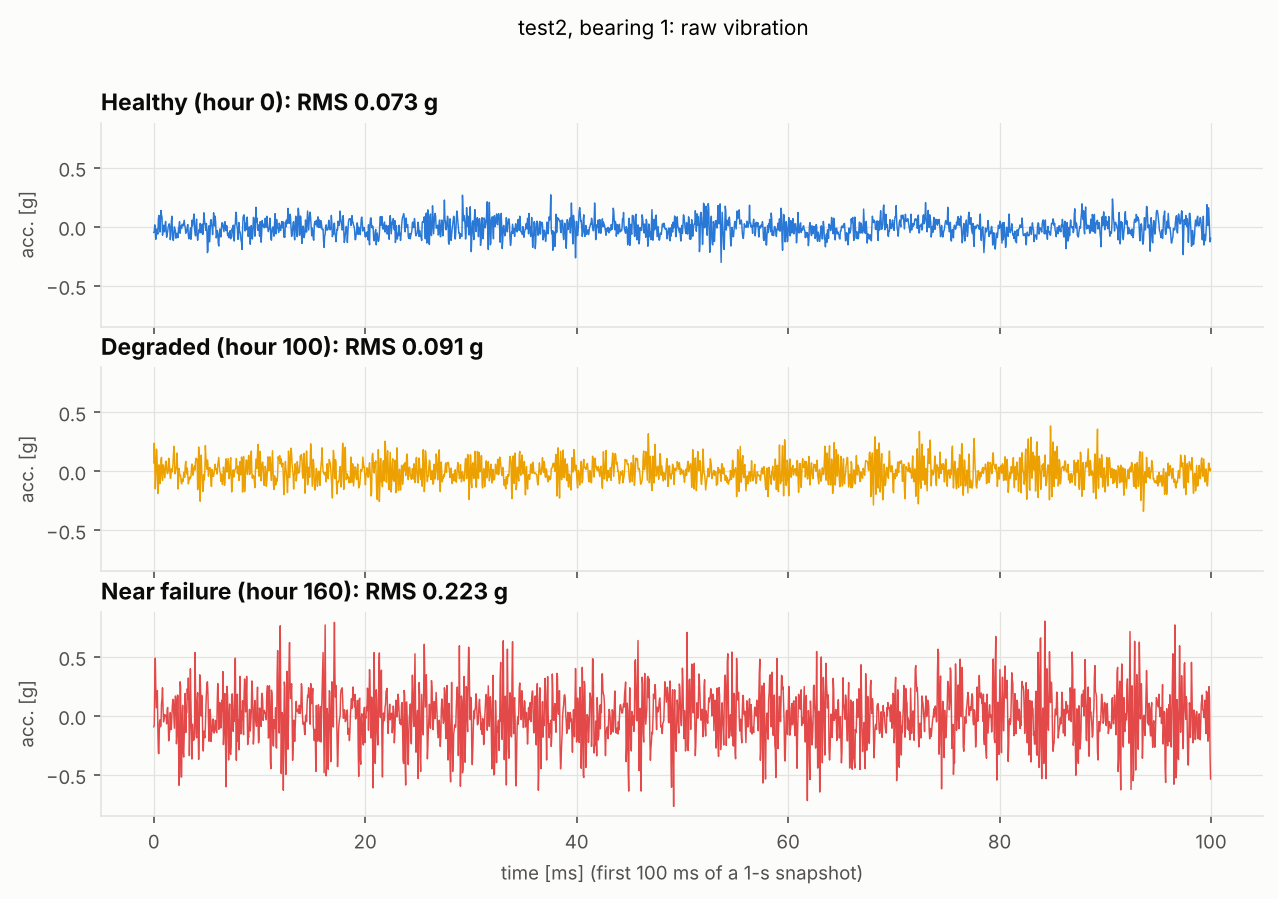
\includegraphics[width=0.92\figw]{report_waveforms.png}
\caption{Test~2, rulman~1'in ham titreşimi (üç kaydın ilk 100\,ms'si).}
\label{fig:wave}
\end{figure}

\textbf{Yorum.} 100.\ saatte dalga biçimi görsel olarak sağlıklı olana hâlâ benzer ve RMS yalnızca
0,073'ten 0,091\,g'ye (+\%25) çıkmıştır; bu artış gözle veya sabit bir titreşim sınırıyla kolayca
gözden kaçabilir. Arızaya yakın dönemde genlik üç katına çıkmış (0,223\,g) ve sinyal belirgin biçimde
darbeli hâle gelmiştir. Dolayısıyla erken uyarı, dalga biçimine bakmaktan veya toplam seviyeden fazlasına
dayanmalıdır.

\begin{figure}[H]
\centering
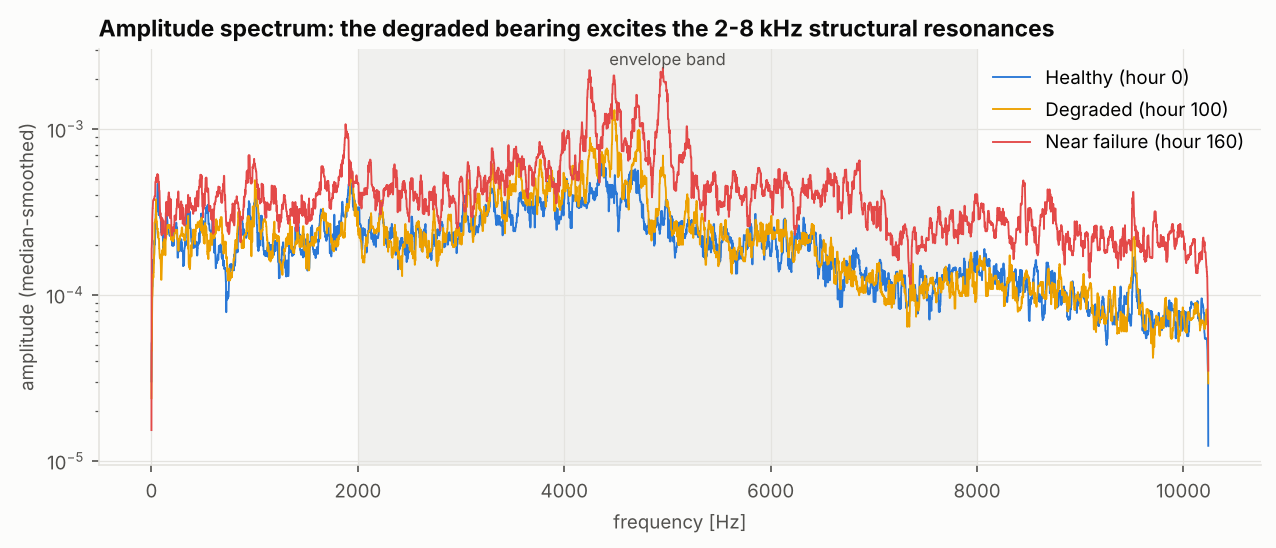
\includegraphics[width=0.92\figw]{report_spectrum.png}
\caption{Aynı üç kaydın genlik spektrumu (medyan filtreyle yumuşatılmış, logaritmik ölçek).}
\label{fig:spec}
\end{figure}

\textbf{Yorum.} Üç spektrumun da enerjisi yaklaşık 3 ile 6\,kHz arasında toplanır: bunlar rulman
gövdesinin yapısal rezonanslarıdır. Rulman bozuldukça rezonans tepeleri büyür ve genişler; arızaya
yakın dönemde yüksek frekans tabanı (6--10\,kHz) neredeyse bir mertebe yükselir. Bu durum hem göreli
bant enerjisi özniteliklerini hem de zarf analizi için 2--8\,kHz bandının seçimini doğrular. Ancak
spektrum, \emph{hangi} parçanın hasarlı olduğunu göstermez.

\begin{figure}[H]
\centering
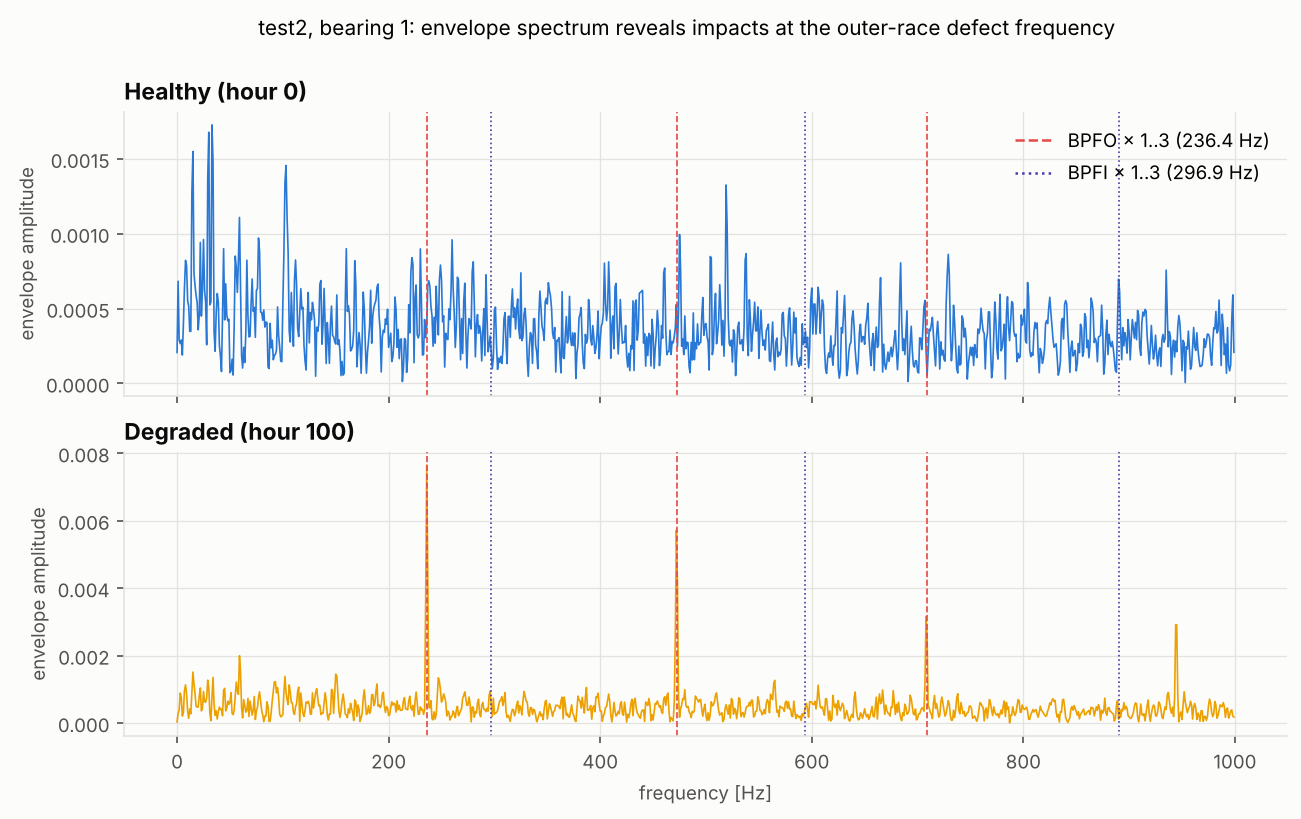
\includegraphics[width=0.92\figw]{report_envelope.png}
\caption{Sağlıklı ve bozulmuş kayıtların zarf spektrumu; BPFO'nun (kesikli) ve BPFI'nin (noktalı) ilk üç
harmoniği işaretlenmiştir.}
\label{fig:env}
\end{figure}

\textbf{Yorum.} Bu, teşhis açısından en önemli şekildir. Sağlıklı zarf spektrumu, arıza
frekanslarında hiçbir yapı içermeyen düz bir gürültü tabanıdır. 100.\ saatte tam olarak 236, 473 ve
709\,Hz'de, yani BPFO'nun $1\times$, $2\times$ ve $3\times$ katlarında, gürültü tabanının yaklaşık on
katı genlikte keskin tepeler belirir; iç bilezik frekanslarında ise hiçbir şey görünmez. Bu, lokal bir
\textbf{dış bilezik} hasarının ders kitabı imzasıdır ve testin bitiminden yaklaşık üç gün önce
görünürdür. Şekil, rulman geometrisinin, arıza frekansı hesabının ve zarf hattının doğru olduğunu
doğrular; \code{env\_bpfo} özniteliğinin ölçtüğü de budur.

\subsection{Ön işleme ve veri bölmeleri}
\label{sec:prep}
Öznitelikler her rulman için bir matrise dönüştürülür (her satır bir kayıt, zaman sırasıyla). Kesin
pozitif ve ağır kuyruklu özniteliklerin logaritması alınır; ardından her öznitelik, o rulmanın kendi
eğitim döneminin ortalaması ve standart sapmasıyla standartlaştırılır (Kod~\ref{lst:prep}). Bu adımdan
sonra $+3$ değeri, rulman doğası gereği gürültülü ya da sessiz olsun, ``bu rulmanın normalinin üç
sağlıklı standart sapma üstü'' anlamına gelir; böylece bir testteki tüm rulmanlar tek bir dedektörle
izlenebilir.

\begin{lstlisting}[caption={Zaman sıralı bölmeler ve rulman bazında standartlaştırma (\code{src/bearing\_efw/preprocess.py}'den alıntı).},label=lst:prep]
for bearing, w in wide_by_bearing(df).items():
    hours = ((w.index - t0).total_seconds() / 3600).to_numpy()
    # Splits use the snapshot index, not wall-clock time: test1 was recorded in
    # bursts with multi-day gaps, so a time-based split would leave almost no
    # training data.
    life = np.arange(len(w)) / len(w)
    train = life < train_end                       # first 25 %
    calib = (life >= train_end) & (life < calib_end)  # next 10 %

    Z = w.copy()
    log_cols = [c for c in Z.columns if c.rsplit("_ch", 1)[0] in LOG_FEATURES]
    Z[log_cols] = np.log(Z[log_cols].clip(lower=1e-9))
    mu, sd = Z[train].mean(), Z[train].std().replace(0, 1)
    X = ((Z - mu) / sd).to_numpy(dtype=np.float32)
\end{lstlisting}

\begin{table}[H]
\centering
\caption{Rulman başına bölme boyutları.}
\label{tab:splits}
\begin{tabular}{lrrrrr}
\toprule
Test & Kayıt & Eğitim & Kalibrasyon & Eğitim bitişi [sa] & Kalibrasyon bitişi [sa] \\
\midrule
test1 & 2\,156 & 539   & 216 & 290,1 & 433,8 \\
test2 & 982    & 246   & 98  & 40,8  & 57,2 \\
test3 & 6\,323 & 1\,581 & 633 & 267,5 & 380,2 \\
\bottomrule
\end{tabular}
\end{table}

\subsection{Dedektörler}
Tüm dedektörler ortak bir arayüze sahiptir: \code{fit} dört rulmanın sağlıklı eğitim matrislerinin
listesini alır, \code{score} ise bir rulmanın tüm matrisini kayıt başına bir puana dönüştürür. Tüm
rulmanların standartlaştırılmış sağlıklı verisini birleştirerek eğitmek, rulman başına ayrı model
eğitmeye göre eğitim kümesini dört katına çıkarır.

\begin{lstlisting}[caption={Klasik dedektörler (\code{src/bearing\_efw/models.py}'den alıntı).},label=lst:models]
class RMSThreshold:
    """Classic condition-monitoring baseline: overall vibration level (z-score of log RMS)."""
    def fit(self, Xs): return self
    def score(self, X): return X[:, self.idx].max(axis=1)   # idx = RMS columns

class Mahalanobis:
    """Distance from the healthy feature distribution (shrinkage covariance)."""
    def fit(self, Xs):
        self.cov = LedoitWolf().fit(np.vstack(Xs))
        return self
    def score(self, X):
        return np.sqrt(self.cov.mahalanobis(X))

class IForest:
    def __init__(self, n_estimators=300, seed=0):
        self.model = IsolationForest(n_estimators=n_estimators, random_state=seed)
    def fit(self, Xs):
        self.model.fit(np.vstack(Xs))
        return self
    def score(self, X):
        return -self.model.score_samples(X)   # higher = more anomalous
\end{lstlisting}

\paragraph{LSTM otokodlayıcı mimarisi.} Kodlayıcı LSTM (32 gizli birim) ardışık $W=12$ kayıttan
(yaklaşık iki saat) oluşan bir pencereyi okur; son gizli durumu 8 boyutlu bir gizli koda izdüşürülür.
Kod çözücü bu kodu 12 adım boyunca tekrarlar, ikinci bir LSTM (32 birim) ve doğrusal bir katmandan
geçirerek öznitelik boyutuna geri döndürür. Model 18 öznitelik için 16\,250 (test~1'in 36 özniteliği
için 19\,148) parametreye sahiptir. Model Adam ile (öğrenme oranı $2\times10^{-3}$, yığın boyutu 64) 60
epok boyunca \emph{gürültü giderici} (denoising) otokodlayıcı olarak eğitilir: girdiye standart sapması
0,1 olan Gauss gürültüsü eklenir ve modelden temiz pencereyi yeniden oluşturması istenir. Yalnızca
yaklaşık 1\,000 pencerelik bir eğitim kümesinde (test~2) bu, ağın eğitim verisini ezberlemesini önler.
Pencereler rulman bazında oluşturulur, hiçbir zaman iki rulmanı kapsamaz ve $t$ kaydının penceresi $t$'de
biter; dolayısıyla puan yalnızca geçmiş veriyi kullanır ve çevrimiçi (online) çalışabilir.

\begin{lstlisting}[caption={LSTM otokodlayıcı (\code{src/bearing\_efw/models.py}'den alıntı).},label=lst:lstm]
class Net(nn.Module):
    def __init__(self):
        super().__init__()
        self.enc = nn.LSTM(n_features, hidden, batch_first=True)
        self.to_latent = nn.Linear(hidden, latent)
        self.from_latent = nn.Linear(latent, hidden)
        self.dec = nn.LSTM(hidden, hidden, batch_first=True)
        self.out = nn.Linear(hidden, n_features)

    def forward(self, x):                       # x: (batch, window, features)
        _, (h, _) = self.enc(x)
        z = self.to_latent(h[-1])               # latent code
        rep = self.from_latent(z).unsqueeze(1).repeat(1, x.shape[1], 1)
        y, _ = self.dec(rep)
        return self.out(y)

def fit(self, Xs):
    # Windows are built per bearing so a sequence never spans two bearings.
    W = torch.tensor(np.concatenate([self._windows(X)[self.window - 1:] for X in Xs]))
    opt = torch.optim.Adam(self.net.parameters(), lr=self.lr)
    for _ in range(self.epochs):
        for idx in np.array_split(self.rng.permutation(len(W)), max(1, len(W) // self.batch_size)):
            xb = W[idx]
            # denoising objective: reconstruct the clean window from a noisy copy
            loss = ((self.net(xb + self.noise * torch.randn_like(xb)) - xb) ** 2).mean()
            opt.zero_grad(); loss.backward(); opt.step()

def score(self, X):
    with torch.no_grad():
        W = torch.tensor(self._windows(X))       # window ending at each snapshot
        return ((self.net(W) - W) ** 2).mean(dim=(1, 2)).numpy()
\end{lstlisting}

\subsection{Puandan alarma}
\paragraph{Eşik.} Her rulman ve dedektör için eşik yalnızca kalibrasyon puanlarından ($s$) türetilir:
\begin{equation}
\tau = Q_{0.995}(s) + m\,\bigl(Q_{0.995}(s) - \operatorname{medyan}(s)\bigr), \qquad m = 0{,}5.
\end{equation}
Pay (margin), sağlıklı puanların yayılımına göre ifade edildiğinden kural her ölçek ve işaretteki puan
için çalışır (RMS z-puanı negatif olabilir, diğer puanlar olamaz).

\paragraph{Debounce.} Eşiği aşan tek bir gürültülü kayıt operatörü uyarmamalıdır. Son $n=6$ kaydın
(bir saat) en az $k=4$'ü $\tau$'yu aştığında $t$ anında alarm etkindir.

\paragraph{Kalıcı alarm.} Gerçek bir bozulma kendiliğinden düzelmez. Arızalı bir rulman için raporlanan
uyarı, kaydın sonuna kadar sürmesi şartıyla \emph{son} alarm bölümünün başlangıcıdır; daha önce
başlayıp sona eren bölümler ayrıca sayılır.

\begin{lstlisting}[caption={Eşik, k-of-n debounce ve kalıcı alarm (\code{src/bearing\_efw/alarm.py}).},label=lst:alarm]
def fit_threshold(calib_scores, quantile, margin):
    q, med = np.quantile(calib_scores, quantile), np.median(calib_scores)
    return float(q + margin * (q - med))

def k_of_n(exceed: np.ndarray, k: int, n: int) -> np.ndarray:
    """Alarm at t when at least k of the last n snapshots (inclusive) exceed the threshold."""
    c = np.convolve(exceed.astype(int), np.ones(n, dtype=int))[: len(exceed)]
    return c >= k

def first_persistent_alarm(alarm, hours, start_h):
    """Start of the final alarm episode, if it lasts until the end of the record."""
    eps = [(s, e) for s, e in alarm_episodes(alarm) if hours[s] >= start_h]
    if not eps:
        return None
    return float(hours[eps[-1][0]]) if eps[-1][1] == len(alarm) else None
\end{lstlisting}

\subsection{Teşhis}
Kalıcı bir alarm verildiğinde sistem, alarm veren rulmanın standartlaştırılmış zarf özniteliklerine
sonraki 12 kayıt boyunca bakar ve ortalama z-puanı en yüksek olan arıza frekansını, 3'ü aşıyorsa,
raporlar (Kod~\ref{lst:diag}). Aksi hâlde tahmin yürütmek yerine ``belirgin arıza frekansı yok'' der.

\begin{lstlisting}[caption={Zarfa dayalı teşhis (\code{scripts/run\_experiment.py}'den alıntı).},label=lst:diag]
DEFECTS = {"env_bpfo": "outer race", "env_bpfi": "inner race", "env_bsf": "rolling element"}

def diagnose(d, alarm_h, n=12):
    if alarm_h is None:
        return ""
    cols = list(d.raw.columns)
    after = np.flatnonzero(d.hours >= alarm_h)[:n]
    z = {k: np.mean([d.X[after, cols.index(c)].mean() for c in cols if c.startswith(k + "_")])
         for k in DEFECTS}
    best = max(z, key=z.get)
    return f"{DEFECTS[best]} (z={z[best]:.1f})" if z[best] > 3 else "no clear defect frequency"
\end{lstlisting}

\subsection{Değerlendirme protokolü}
Veri seti yalnızca her test durdurulduğunda bir rulmanın arızalı olduğunu belirtir; bozulmanın
başlangıcı etiketli değildir. Buradan iki metrik çıkar:
\begin{itemize}
  \item Arızalı bir rulmanın \textbf{uyarı süresi}: kalıcı alarmı ile testin bitişi arasındaki saat
        (test süresinin yüzdesi olarak da verilir). Yüksek olması daha iyidir.
  \item \textbf{Yanlış alarmlar}: sağlıklı olduğuna inanılan bir pencere içinde \emph{herhangi bir}
        rulmanda verilen alarm bölümleri. Bu pencere kalibrasyondan sonra (kayıtların \%35'i) başlar ve
        test 1, 2 ve 3 için sırasıyla kayıtların \%60, \%50 ve \%85'inde biter. Bu sınırlar durum
        göstergelerinin incelenmesinden gelir (Bölüm~\ref{sec:results}) ve yapılandırma dosyasında
        belgelenmiştir. Oran, bu penceredeki 1\,000 rulman-saat başına normalleştirilir.
\end{itemize}
Hiperparametreler (bölme oranları, eşik yüzdeliği ve payı, $k$ ve $n$, ağ boyutu, epok sayısı, gürültü)
yalnızca test~2 üzerinde seçilmiştir. Test~1 ve test~3 hiçbir karar için kullanılmamış ve ayrılmış
değerlendirme kümeleri olarak kalmıştır.

\subsection{Tasarım kararları}
\label{sec:design}
\begin{itemize}
  \item \textbf{Baştan eğit, gerisinde test et.} Tüm bölmeler zaman sıralıdır. Tüm deneyden alınan
        pencereleri karıştırmak arızayı eğitime sızdırır.
  \item \textbf{Bir kayıt, zamanda bir noktadır.} Öznitelikler dosya başına hesaplanır, böylece
        sonuçlar ``arızadan kaç saat önce'' cinsinden ifade edilir.
  \item \textbf{Doğru rulmanı ve her rulmanı izle.} Her rulman ayrı puanlanır; arızalanan rulmanlar
        veri setinin belgelerinden bilinir ve yalnızca değerlendirmede kullanılır.
  \item \textbf{Saate göre değil, kayıt sayısına göre böl.} Test~1'deki çok günlük boşluklar
        nedeniyle \emph{sürenin} ilk \%25'i çok az kayıt içerirdi.
  \item \textbf{Rulman bazında temel seviye.} Her rulmanın kendine göre standartlaştırılması, doğal
        titreşim seviyeleri farklı rulmanların tek bir modelle izlenmesini sağlar.
  \item \textbf{Tüm dedektörler için aynı eşik kuralı ve alarm mantığı}; böylece sonuçlardaki farklar
        ayar farkından değil dedektörlerin kendisinden gelir.
  \item \textbf{Belirlenimcilik (determinism).} Tüm rastgele bileşenler sabit tohumla başlatılır; art
        arda iki çalıştırma aynı sonuç tablolarını üretir.
\end{itemize}

%=====================================================================
\section{Sonuçlar}
\label{sec:results}
%=====================================================================

\subsection{Ana sonuçlar}

\begin{table}[H]
\centering
\caption{Her arızalı rulmanda kalıcı alarmın uyarı süresi (testin bitişinden kaç saat önce) ve yanlış
alarmlar. Kalın: sütundaki en iyi değer.}
\label{tab:results}
\small\setlength{\tabcolsep}{4.5pt}
\begin{tabular}{lrrrrr}
\toprule
 & \multicolumn{2}{c}{test1 (ayrılmış)} & test2 (gelişt.) & test3 (ayrılmış) & Yanlış alarm \\
\cmidrule(lr){2-3}
Dedektör & R3 iç bil. & R4 yuv. el. & R1 dış bil. & R3 dış bil. & / 1000 rulman-sa \\
\midrule
RMS eşiği         & \textbf{99,0} & \textbf{176,6} & 74,3 & \textbf{59,3} & 5,34 \\
Mahalanobis       & 12,2 & 48,0  & 74,3 & 58,7 & 0,67 \\
Isolation Forest  & 12,9 & 156,6 & 72,8 & 14,0 & \textbf{0,00} \\
LSTM otokodlayıcı & 84,9 & 156,6 & \textbf{74,7} & 58,3 & 12,67 \\
\bottomrule
\end{tabular}
\end{table}

\begin{table}[H]
\centering
\caption{Test başına yanlış alarm bölümleri ve değerlendirme penceresinin boyutu.}
\label{tab:fa}
\begin{tabular}{lrrr}
\toprule
Dedektör & test1 & test2 & test3 \\
\midrule
RMS eşiği         & 15 & 0 & 1 \\
Mahalanobis       & 0  & 0 & 2 \\
Isolation Forest  & 0  & 0 & 0 \\
LSTM otokodlayıcı & 4  & 2 & 32 \\
\midrule
Sağlıklı pencere (saat)        & 434--632 & 57--82 & 380--908 \\
Sağlıklı pencere (rulman-saat) & 3\,162 & 389 & 8\,443 \\
\bottomrule
\end{tabular}
\end{table}

\begin{figure}[H]
\centering
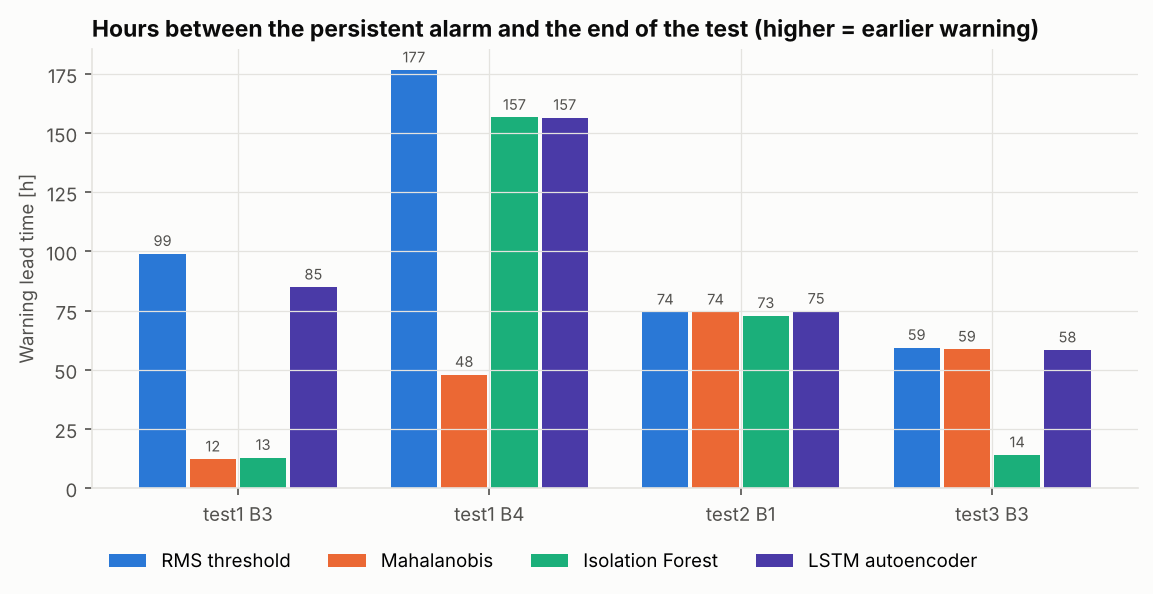
\includegraphics[width=0.95\figw]{lead_times.png}
\caption{Her arızalı rulman ve dedektör için kalıcı alarmın uyarı süresi.}
\label{fig:lead}
\end{figure}

\textbf{Şekil~\ref{fig:lead}'in yorumu.} Test~2'de dört sütun pratikte eşittir (73--75\,sa): bir hasar
temiz biçimde geliştiğinde makul her dedektör onu aynı anda görür ve dedektör seçimi önemli değildir.
Ayrılmış testler dedektörleri birbirinden ayırır. Test~1'de RMS temel modeli ve LSTM otokodlayıcı en
erken uyarıyı verir (85--177\,sa); Mahalanobis uzaklığı ise bitişten yalnızca 12--48\,sa önce uyarır.
Test~3'te üç dedektör yaklaşık 59\,sa, Isolation Forest ise yalnızca 14\,sa verir. Tablo~\ref{tab:fa}
ile birlikte okunduğunda, en erken uyaran dedektörlerin aynı zamanda en çok yanlış alarm üreten
dedektörler olduğu görülür; bedava öğle yemeği yoktur.

\subsection{Test 2 (geliştirme kümesi)}

\begin{figure}[H]
\centering
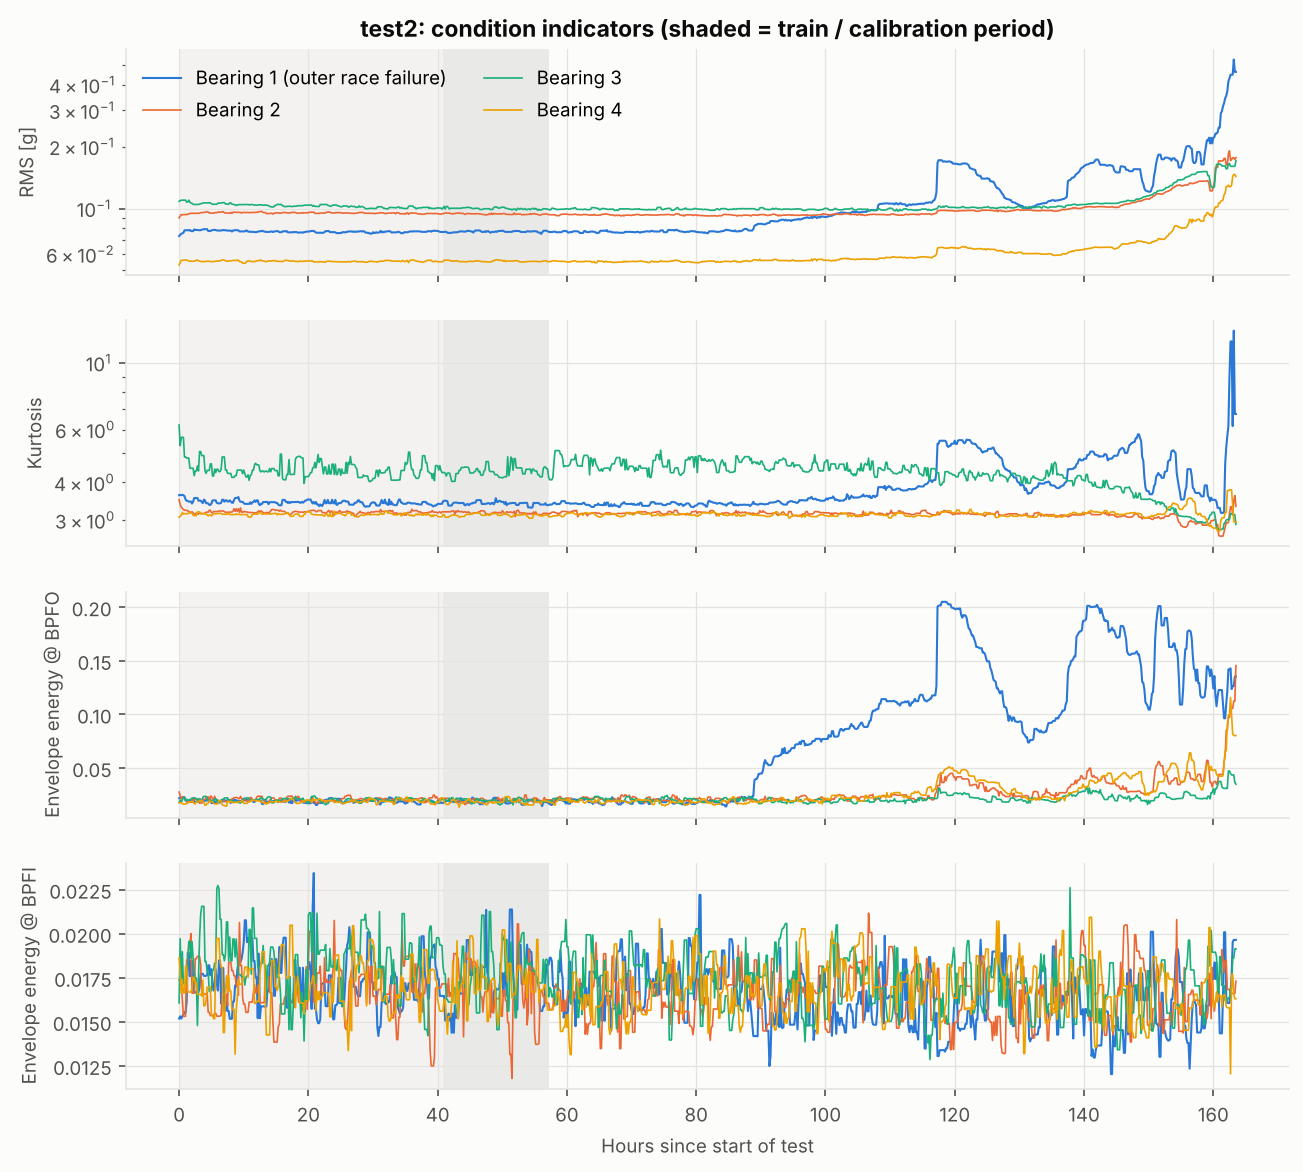
\includegraphics[width=0.93\figw]{test2_indicators.png}
\caption{Test~2'nin durum göstergeleri (5 kayıtlık kayan medyan). Gölgeli alanlar: eğitim ve kalibrasyon
dönemleri.}
\label{fig:t2ind}
\end{figure}

\textbf{Yorum.} İlk 85 saat boyunca dört rulmanın tüm göstergeleri düzdür. Yaklaşık 88.\ saatte
rulman~1'in BPFO zarf enerjisi 0,02'den 0,05'e sıçrar ve 118.\ saatte yaklaşık 0,2'ye kadar yükselmeye
devam eder; RMS ise yalnızca yavaşça artar. Bu, Şekil~\ref{fig:env}'de görülen dış bilezik hasarıdır.
Rulman~1'in basıklığı da (darbeler) artar, ancak daha kademeli olarak. BPFI zarf enerjisi tüm rulmanlar
için gürültü seviyesinde kalır; bu, iç bilezik değil dış bilezik hasarıyla tutarlıdır. Yaklaşık 115.\
saatten itibaren diğer rulmanların RMS'i ve BPFO enerjisi de artar: rulman~1'in titreşimi mil ve gövde
üzerinden diğerlerine iletilir. Son saatlerde tüm göstergeler dik biçimde yükselir. Rulman~1'in BPFO
enerjisinin 130.\ saat civarındaki ``çukuru'' oyuk (spall) gelişiminde tipiktir: hasarın kenarları
aşınıp yumuşadıkça darbeler geçici olarak zayıflar, ardından hasar yayılır.

\begin{figure}[H]
\centering
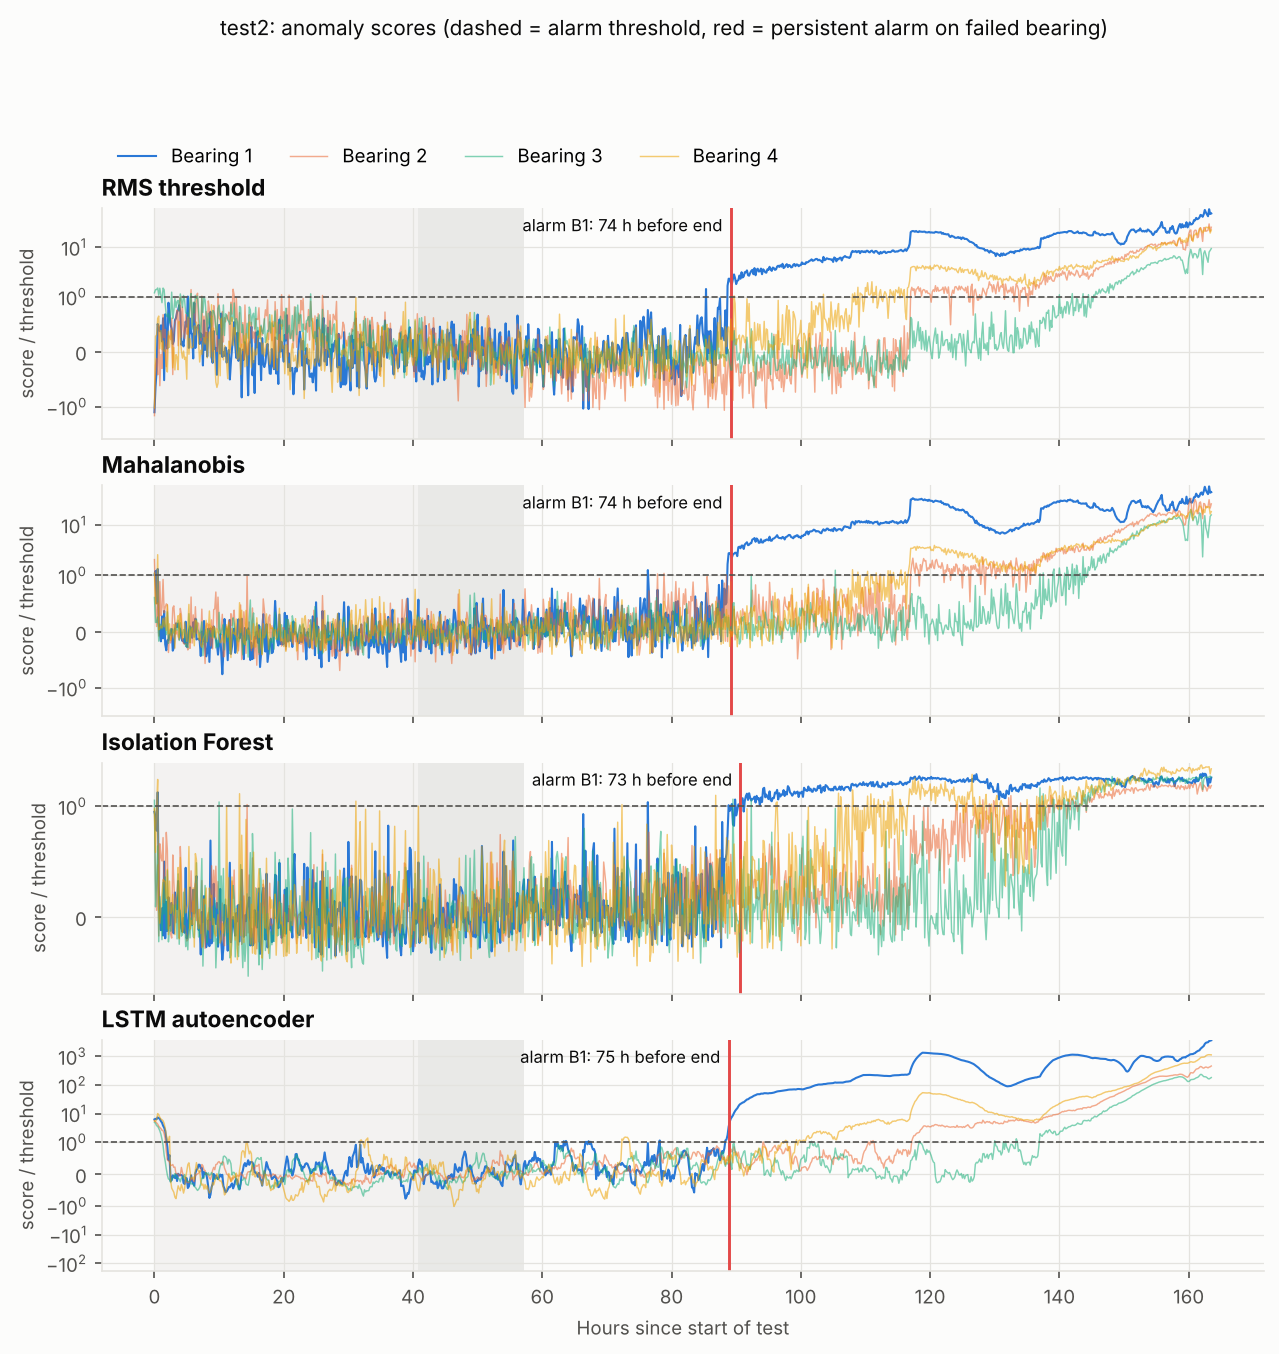
\includegraphics[width=0.93\figw]{test2_detectors.png}
\caption{Test~2 anomali puanlarının her rulmanın eşiğine oranı (simetrik log ölçek). Kesikli çizgi: alarm
eşiği; kırmızı çizgi: arızalı rulmandaki kalıcı alarm.}
\label{fig:t2det}
\end{figure}

\textbf{Yorum.} Dört dedektör de eğitim, kalibrasyon ve sonraki 30 saat boyunca tüm rulmanları eşiğin
altında tutar; ardından rulman~1 89.\ saatte eşiği aşar ve bir daha altına inmez: bitişten 74 saat önce
kalıcı alarm. Puan sıçraması tüm öznitelikleri birleştiren LSTM otokodlayıcıda (iki mertebe) ve
Mahalanobis uzaklığında (yaklaşık $20\times$) en büyük, puanı yapısı gereği doygunluğa ulaşan Isolation
Forest'ta en küçüktür. İki kısa LSTM bölümü (yanlış alarm olarak sayılır) dışında diğer rulmanlar eşiği
ancak 109--145.\ saatlerden sonra ve her zaman rulman~1'den sonra aşar; dolayısıyla \emph{ilk alarm
veren rulman} kaynağı doğru biçimde gösterir. Tüm dedektörler alarm anında \textbf{dış bilezik} hasarı
teşhis eder (z-puanları 6,1--7,3); bu, belgelenmiş arıza tipidir. Rulman 2 ve 4 de sonraki alarmlarında
dış bilezik teşhisi alır, çünkü rulman~1'in titreşimini taşırlar; panelin ilk alarm veren rulmanı
muhtemel kaynak olarak işaretlemesinin nedeni budur.

\subsection{Test 1 (ayrılmış)}

\begin{figure}[H]
\centering
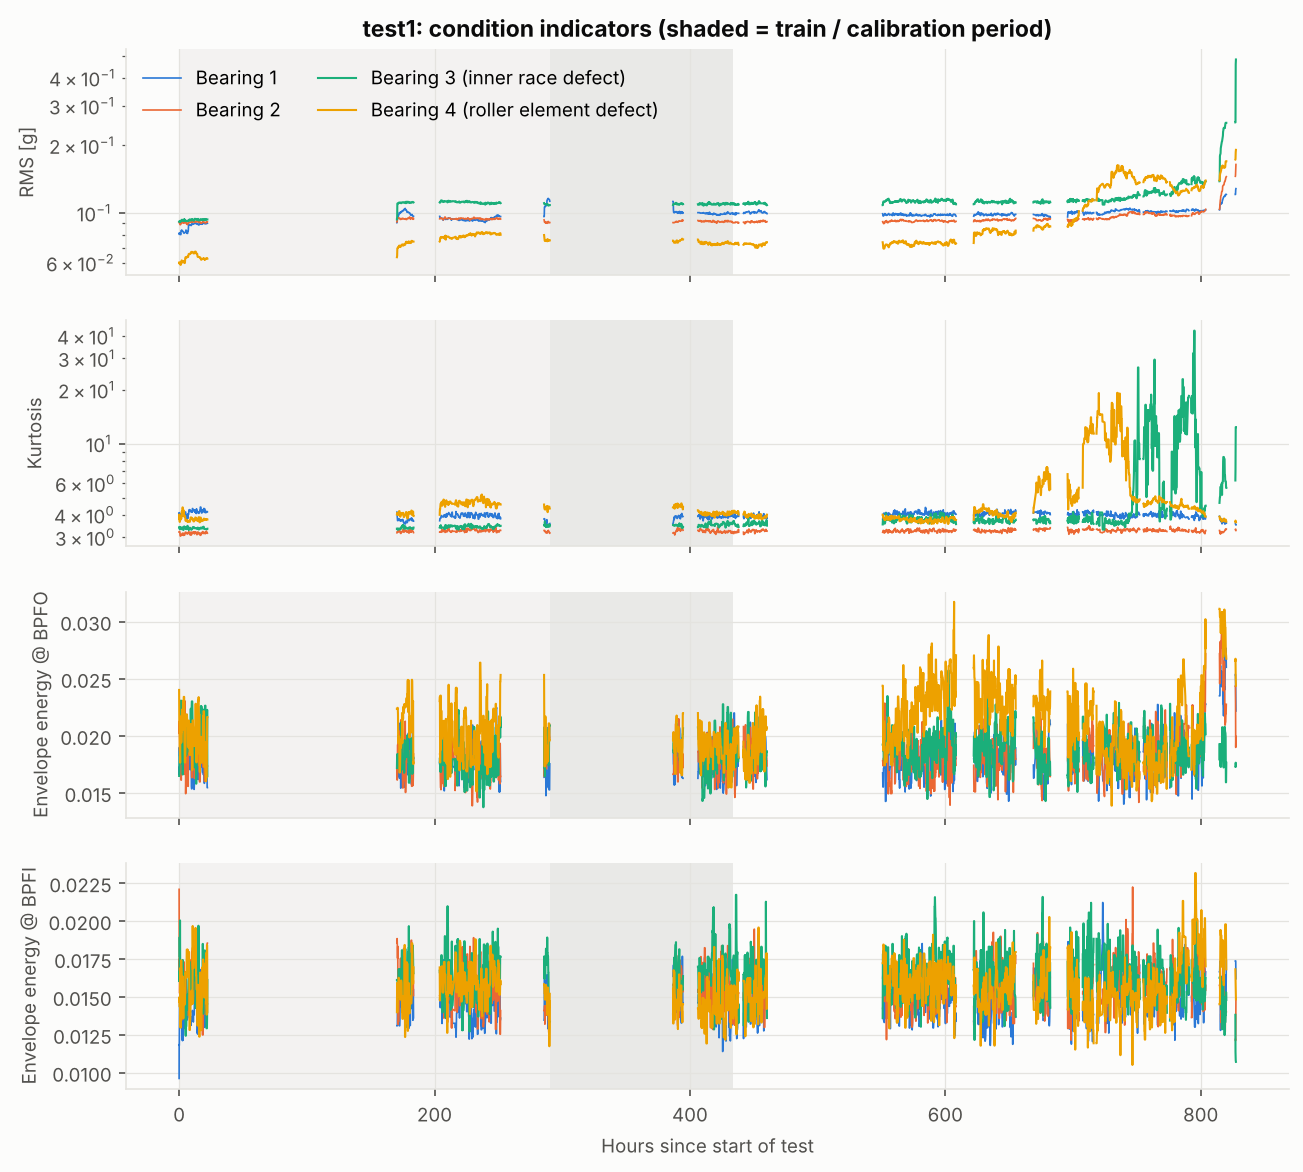
\includegraphics[width=0.93\figw]{test1_indicators.png}
\caption{Test~1'in durum göstergeleri. Çizgi kesintileri kayıt boşluklarıdır.}
\label{fig:t1ind}
\end{figure}

\textbf{Yorum.} Test~1 en zor kayıttır: altı güne varan boşluklarla parçalanmıştır ve eğitim dönemi
(ilk 539 kayıt, 290.\ saate kadar) kayıt parçaları arasında birkaç basamak değişimi içerir; yani
``sağlıklı'' tek ve kararlı bir durum değildir. İki arızalı rulmanın bozulması basıklıkta açıkça
görülür: rulman~4 yaklaşık 680.\ saatten itibaren (basıklık 20'ye kadar), rulman~3 ise yaklaşık 720.\
saatten itibaren (40'a kadar) darbeli hâle gelir; bu, RMS'leri artmadan çok öncedir. BPFI'deki zarf
enerjisi (rulman~3'ün iç bilezik hasarı) hiç artmaz, rulman~4'ün BPFO enerjisi de yalnızca dalgalanır.
İç bilezik ve yuvarlanma elemanı hasarları yük bölgesine girip çıktıkları için zarf enerjilerini tek
bir çizgide toplamak yerine $\pm f_r$ ve kafes frekansındaki yan bantlara yayarlar; harmoniklerin
çevresindeki $\pm3$\,Hz'lik pencere bu enerjinin çoğunu kaçırır.

\begin{figure}[H]
\centering
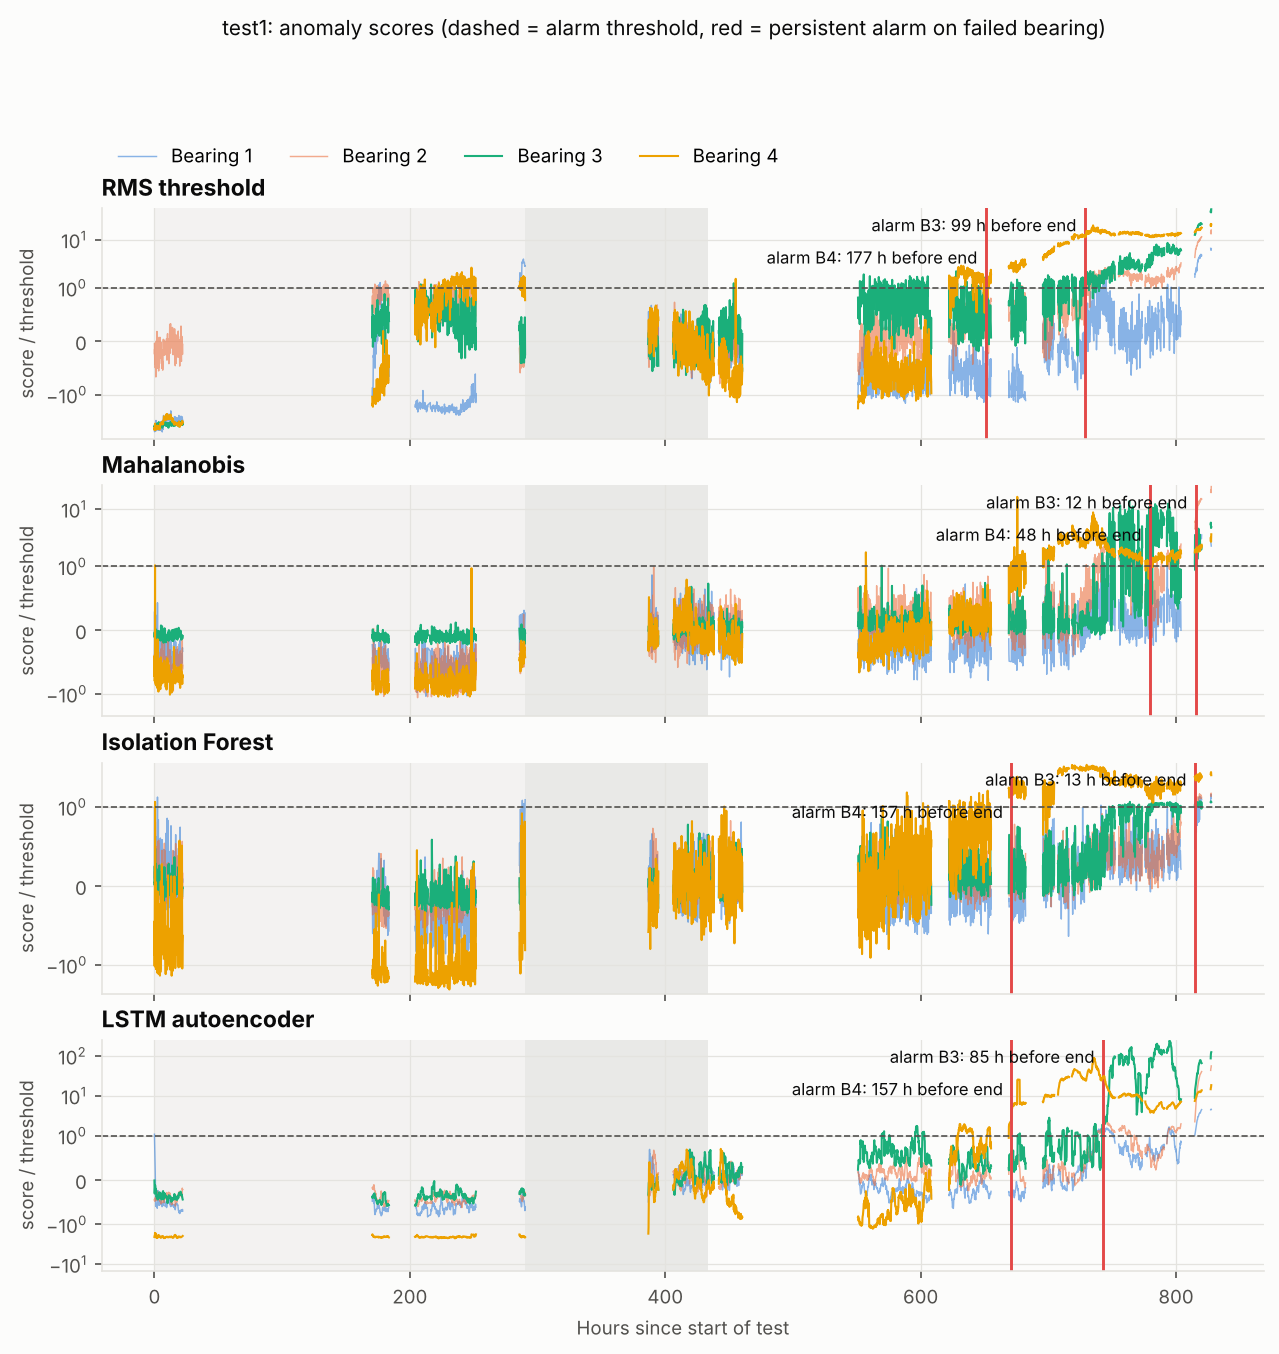
\includegraphics[width=0.93\figw]{test1_detectors.png}
\caption{Test~1 anomali puanlarının her rulmanın eşiğine oranı.}
\label{fig:t1det}
\end{figure}

\textbf{Yorum.} Rulman~4, üç dedektör tarafından bitişten 157--177 saat önce (deneyin \%19--21'i)
tespit edilir ve her dedektör için ilk alarm veren rulmanlar iki arızalı rulmandır; yani kaynak tespiti
doğrudur. RMS temel modeli en erken uyarıyı verir, ancak sağlıklı kabul edilen pencere içinde (434--632.\
saatler) eşiği etrafında salınarak rulman~3'te (554.\ saatten itibaren) ve rulman~4'te (623.\ saatten
itibaren) toplam 15 alarm bölümü üretir. Bunlar tam da daha sonra arızalanan iki rulman olduğu için bu
bölümlerin bir kısmı aslında yanlış alarm değil, bozulmanın ilk işaretleri olabilir; etiketli bir
başlangıç olmadığından değerlendirme bunları temkinli biçimde yanlış alarm sayar. Mahalanobis uzaklığı
ve Isolation Forest hiç yanlış alarm vermez, ancak rulman~3'teki kalıcı alarmları bitişten yalnızca
12--13\,sa önce başlar: aslında eşiği çok daha önce aşmışlardır (rulman~3 için ilk alarm 747.\ ve 756.\
saatlerde), fakat puan yeniden eşiğin altına indiği için temkinli ``kalıcı alarm'' tanımı bu uyarıları
dışarıda bırakır. Bu testte en iyi denge LSTM otokodlayıcıdadır (85\,sa ve 157\,sa, 4 yanlış alarm
bölümü). Yukarıda açıklanan nedenle hiçbir dedektör test~1'de güvenilir bir arıza tipi teşhisi
üretmez.

\subsection{Test 3 (ayrılmış)}

\begin{figure}[H]
\centering
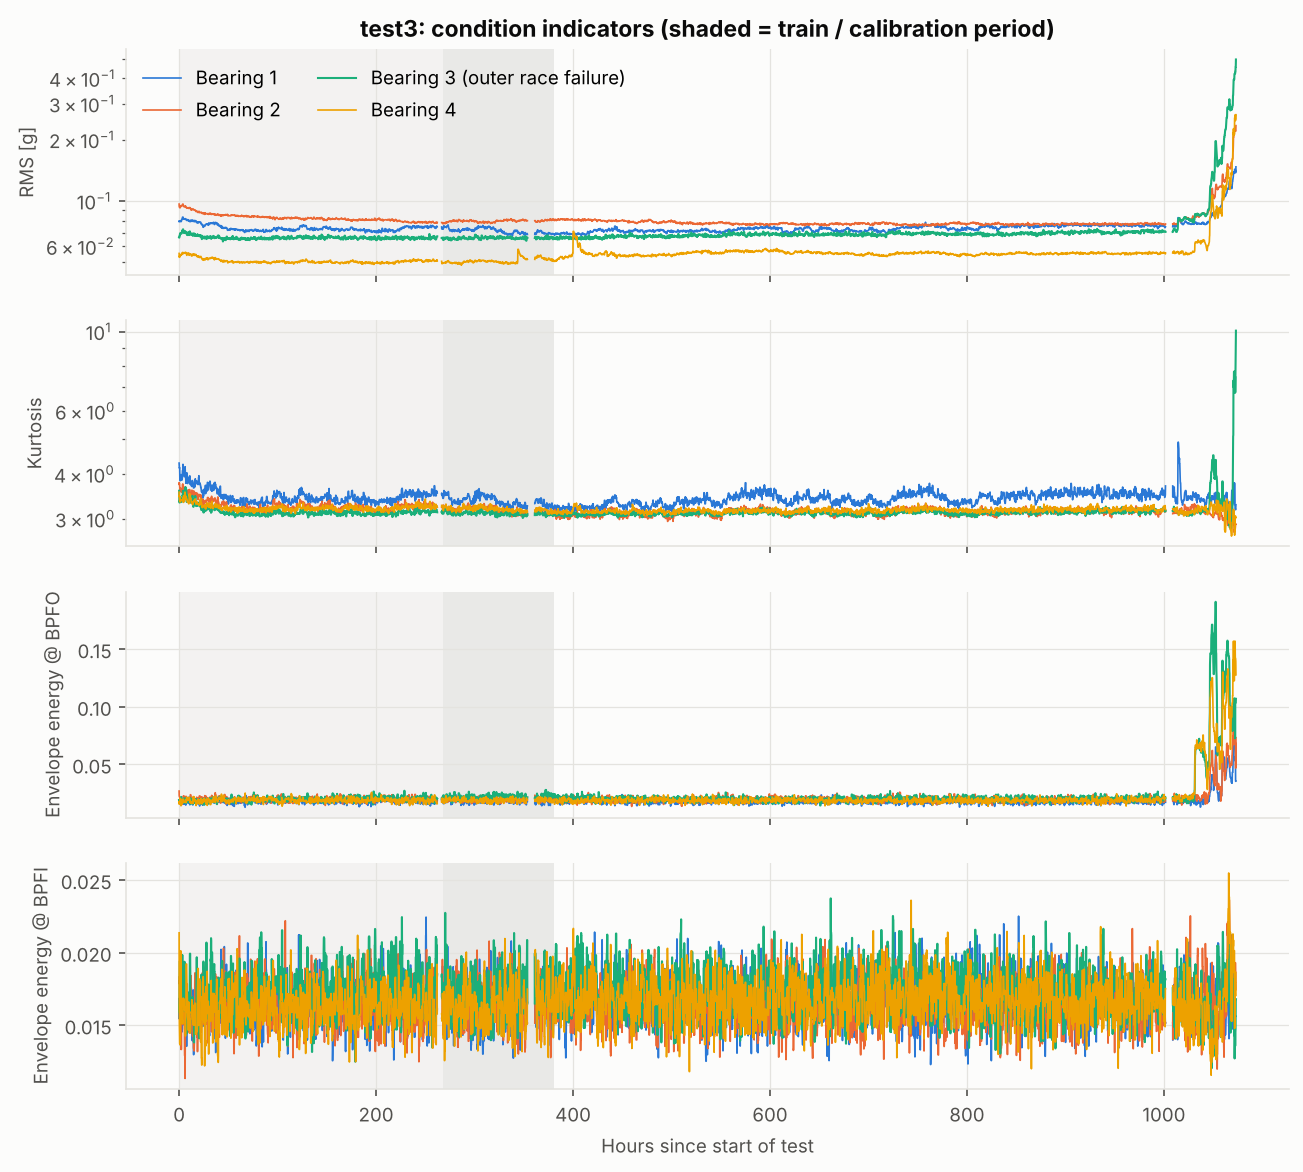
\includegraphics[width=0.93\figw]{test3_indicators.png}
\caption{Test~3'ün durum göstergeleri.}
\label{fig:t3ind}
\end{figure}

\textbf{Yorum.} Test~3 1\,000 saat boyunca neredeyse hiç bozulma belirtisi göstermez. İki olay
önemlidir. Birincisi, 354.\ saat civarındaki 7,5 saatlik duruştan sonra tüm rulmanların RMS'i hafifçe
kayar ve rulman~4 yaklaşık 400.\ saatte kısa bir sıçrama gösterir: makine biraz farklı bir koşulda
yeniden çalışmaya başlamıştır. İkincisi, 1\,002.\ saatteki 7,3 saatlik duruştan sonra tüm göstergeler
değişir ve yaklaşık 1\,040.\ saatten itibaren rulman~3'ün (ve iletim yoluyla rulman~4'ün) BPFO zarf
enerjisi keskin biçimde yükselir; son 20 saatte bunu RMS ve basıklık izler. Dolayısıyla rulman~3'teki
dış bilezik hasarı 44 günlük bir deneyin yalnızca son \%5'inde görünür hâle gelir.

\begin{figure}[H]
\centering
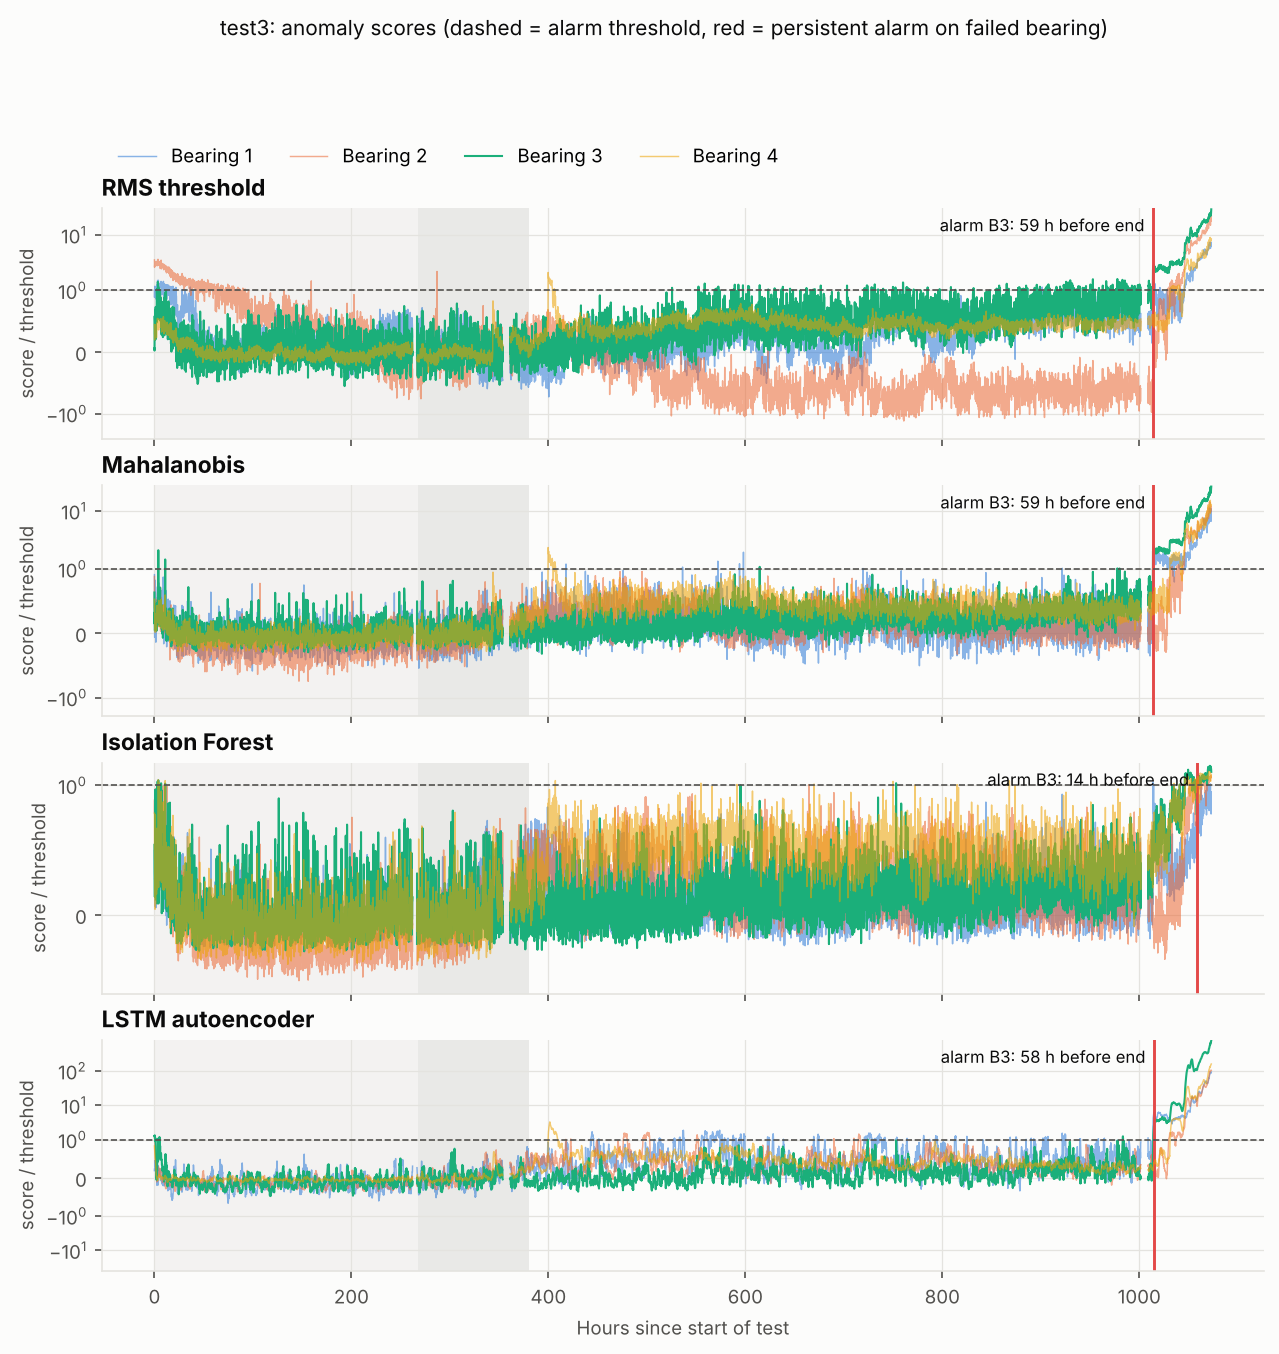
\includegraphics[width=0.93\figw]{test3_detectors.png}
\caption{Test~3 anomali puanlarının her rulmanın eşiğine oranı.}
\label{fig:t3det}
\end{figure}

\textbf{Yorum.} RMS, Mahalanobis ve LSTM dedektörleri rulman~3'te bitişten yaklaşık 59\,sa önce kalıcı
alarm verir; ancak bu alarm duruştan sonra kaydın yeniden başlamasından (1\,009.\ saat) yaklaşık 5 saat
sonra başlar ve rulman~1'deki alarmlarla çakışır. Dolayısıyla bu alarmın bir kısmı hasara değil yeniden
başlatmaya verilen tepkidir ve bu dedektörler hangi rulmanın arızalandığını ayırt edemez (rulman 1 ve 3
aynı kayıtta alarm verir). Alarmı açıkça hasardan kaynaklanan tek dedektör Isolation Forest'tır:
BPFO enerjisi sıçradığında, bitişten 14\,sa önce alarm verir ve 11,4 z-puanıyla \textbf{dış bilezik}
hasarı teşhis eder. 354.\ saatten sonraki rejim değişimi yanlış alarmların ana kaynağıdır: tüm
özniteliklerin ortak değişimini modelleyen LSTM otokodlayıcı yeni temel seviyeyi anormal olarak yorumlar
ve çoğu rulman~1'de olmak üzere 32 bölüm üretir. Bu, deneyin başında bir kez eğitilen bir modelin en
önemli sınırlamasıdır.

\subsection{Bulguların özeti}
\begin{enumerate}
  \item \textbf{Hasar temiz biçimde geliştiğinde erken uyarı çalışır.} Test~2'de tüm dedektörler
        bitişten 74\,sa (deneyin \%45'i) önce uyarır ve doğru arıza tipini belirtir.
  \item \textbf{Uyarı süresi ile yanlış alarm arasında ödünleşim vardır.} RMS temel modeli ve LSTM
        otokodlayıcı en erken uyarır; Isolation Forest hiç yanlış alarm vermemiş ama dört arızanın
        ikisinde geç uyarmıştır; Mahalanobis uzaklığı çok az yanlış alarmla arada yer alır.
  \item \textbf{Güçlü bir temel model önemlidir.} Basit RMS eşiği uyarı süresinde rekabetçidir. Yalnızca
        üç deney içeren bir veri setinde derin model üstünlük kurmaz.
  \item \textbf{İlk alarmla kaynak tespiti} test~1 ve test~2'de güvenilirdir, ancak test~3'teki yeniden
        başlatmadan sonra değildir.
  \item \textbf{Zarf teşhisi dış bilezik hasarları için güvenilirdir} (test~2 ve test~3), ancak mevcut
        dar bantlı öznitelikle test~1'in iç bilezik ve yuvarlanma elemanı hasarlarını tanımaz.
  \item \textbf{Çalışma koşulu değişiklikleri} (yeniden başlatma, bakım) geçerliliğe yönelik ana
        tehdittir: ömrün başında bir kez eğitilen bir model yeni bir normali anomali olarak görür.
\end{enumerate}

%=====================================================================
\section{Etkileşimli Panel (Dashboard)}
%=====================================================================
Sistemin bir operatöre nasıl görüneceğini göstermek için \code{app/dashboard.py} herhangi bir testi
makineden canlı veri geliyormuş gibi yeniden oynatır (Şekil~\ref{fig:dash}). Kullanıcı bir test ve bir
dedektör seçip \emph{Play}'e basar; panel kayıt kayıt ilerler ve şunları gösterir:
\begin{itemize}
  \item her rulman için renk, simge ve etiketle bir durum kartı (sağlıklı / eşik üstünde / alarm),
        puan/eşik oranı, mevcut alarmın başlangıcından bu yana geçen süre, muhtemel kaynak için
        \emph{ilk alarm veren} (first to alarm) işareti ve teşhis edilen arıza tipi;
  \item eğitim ve kalibrasyon dönemleri gölgelenmiş, o ana kadarki tüm rulmanların anomali puanı
        grafiği;
  \item seçilen rulman için BPFO, BPFI ve BSF'deki zarf z-puanları;
  \item bir alarm günlüğü ve istenirse gerçek durum (hangi rulmanın nasıl arızalandığı).
\end{itemize}

\begin{figure}[H]
\centering
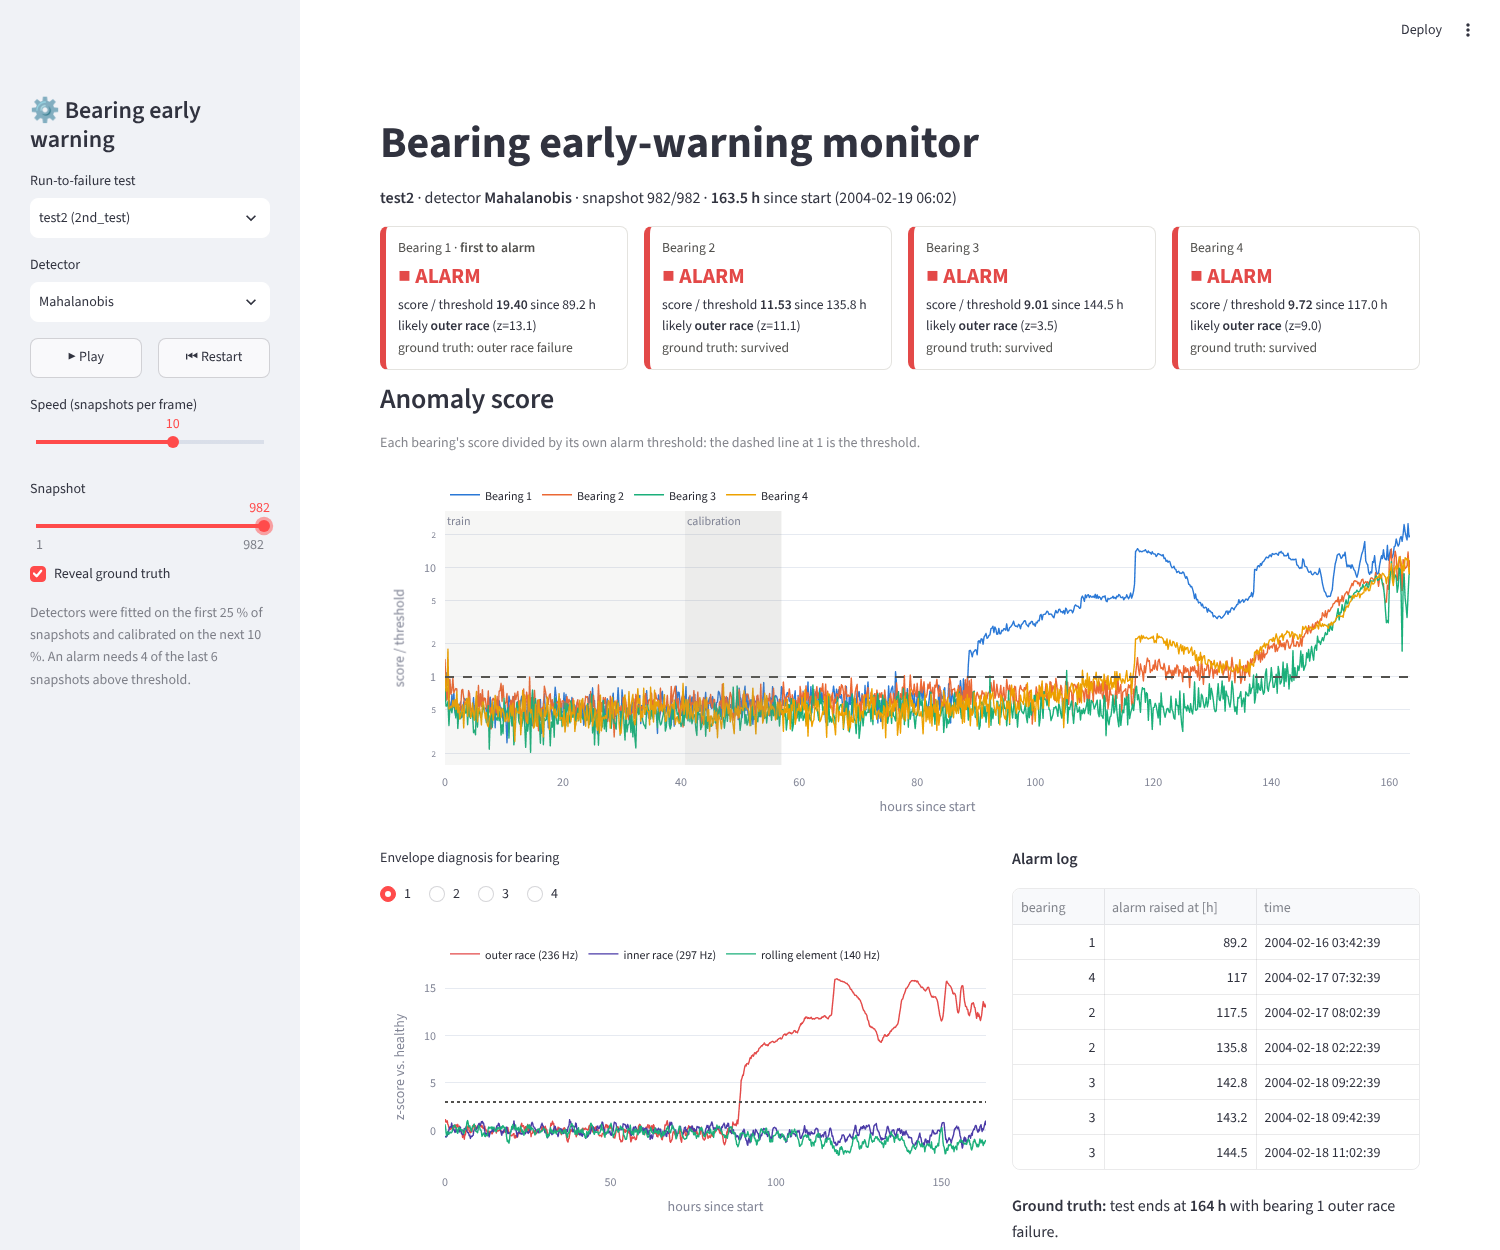
\includegraphics[width=0.95\figw]{dashboard.png}
\caption{Test~2'nin sonunda, Mahalanobis dedektörüyle ve gerçek durum gösterilirken panel.}
\label{fig:dash}
\end{figure}

\textbf{Yorum.} Kartlar test~2'nin hikâyesini tek satırda özetler: rulman~1 belirgin bir dış bilezik
imzasıyla (z = 13,1) ilk alarm veren rulmandır (89,2.\ saatten beri); diğerleri 28--55 saat sonra onu
izler. Zarf grafiği, rulman~1'in BPFO z-puanının 90.\ saat civarında 0'dan 10'un üstüne sıçradığını,
BPFI ve BSF'nin ise düz kaldığını gösterir: teşhisin arkasındaki kanıt operatör tarafından görülebilir.

\begin{lstlisting}[caption={Muhtemel kaynak ve her rulmanın durumu (\code{app/dashboard.py}'den alıntı).},label=lst:dash]
# The first bearing to raise an alarm is the likely source: once it degrades, its
# vibration travels through the shaft and housing and lifts its neighbours too.
onsets = {b: g.loc[g["alarm"], "hours"].min() for b, g in seen.groupby("bearing") if g["alarm"].any()}
source = min(onsets, key=onsets.get) if onsets else None

for col, (b, g) in zip(cols, seen.groupby("bearing")):
    last = g.iloc[-1]
    state = "alarm" if last.alarm else ("watch" if last.score > last.threshold else "ok")
    defect, zval = diagnose(zs[b].loc[:now])      # mean z of the last 6 snapshots
    ...

# Playback: advance the slider and rerun the script
if st.session_state.playing and idx < n:
    st.session_state["advance_to"] = min(n, idx + speed)
    time.sleep(0.15)
    st.rerun()
\end{lstlisting}

Panel yalnızca depoya eklenmiş sonuç dosyalarını okur, bu nedenle ham veri olmadan çalışır:
\code{make dashboard} komutu paneli \code{http://localhost:8501} adresinde açar.

%=====================================================================
\section{Yazılım Mühendisliği ve Yeniden Üretilebilirlik}
%=====================================================================

\subsection{Depo yapısı}
\begin{lstlisting}[style=plain]
configs/default.yaml      splits, thresholds, alarm rule, model hyper-parameters
src/bearing_efw/
    dataset.py            test metadata, bearing geometry, defect frequencies, loader
    features.py           time, spectral and envelope features per snapshot
    preprocess.py         per-bearing matrices, log + standardisation, splits
    models.py             RMS, Mahalanobis, Isolation Forest, LSTM autoencoder
    alarm.py              thresholding, k-of-n debouncing, alarm episodes
    plots.py              report figures
scripts/                  download_data, build_features, run_experiment, make_report_figures
app/dashboard.py          Streamlit replay dashboard
data/features/            extracted features (committed, 3 MB)
reports/                  results.md, summary.csv, scores.csv.gz, figures/
notebooks/                01_walkthrough.ipynb
tests/                    unit tests and dashboard smoke tests
report/                   this report (LaTeX sources and PDFs, English and Turkish)
\end{lstlisting}

\subsection{Yapılandırma}
Deneydeki tüm seçimler tek bir YAML dosyasında tutulur; böylece deney kod değiştirmeden
değiştirilebilir:
\begin{lstlisting}[style=plain]
split:      {train_end: 0.25, calib_end: 0.35}
healthy_end: {test1: 0.60, test2: 0.50, test3: 0.85}
threshold:  {quantile: 0.995, margin: 0.5}
alarm:      {k: 4, n: 6}
models:
  isolation_forest: {n_estimators: 300, seed: 0}
  lstm_ae: {window: 12, hidden: 32, latent: 8, epochs: 60, lr: 0.002,
            batch_size: 64, noise: 0.1, seed: 0}
\end{lstlisting}

\subsection{Çalıştırma}
\begin{lstlisting}[style=plain]
pip install -r requirements.txt
make experiment   # ~2 min, uses the committed feature tables
make dashboard    # interactive replay at http://localhost:8501
make test
make data         # optional: download + extract raw data (~1 GB / 6 GB)
make features     # optional: rebuild the feature tables from raw data
\end{lstlisting}

\subsection{Testler}
On iki otomatik test, sessizce bozulması en olası kısımları denetler. En önemlisi, gürültü içine
gömülmüş ve tam olarak BPFO hızında tekrarlanan rezonans patlamalarından oluşan yapay bir dış bilezik
hasarı üretir ve zarf özniteliğinin bunu tespit edip dış bileziğe atfettiğini kontrol eder
(Kod~\ref{lst:test}). Diğer testler arıza frekanslarını yayımlanmış değerlerle, Gauss gürültüsünün
istatistiklerini (RMS $=1$, basıklık $=3$), debounce ve kalıcılık mantığını, eşiğin puan kaymasına karşı
değişmezliğini ve panelin her test için iki dedektörle hatasız açıldığını denetler.

\begin{lstlisting}[caption={Yapay arıza testi (\code{tests/test\_core.py}'den alıntı).},label=lst:test]
def test_envelope_picks_up_outer_race_impacts():
    """Synthetic outer-race defect: resonance bursts repeating at BPFO."""
    rng = np.random.default_rng(1)
    t = np.arange(FS) / FS
    bpfo = fault_frequencies()["bpfo"]
    impacts = np.zeros(FS)
    impacts[(np.arange(0, 1, 1 / bpfo) * FS).astype(int)] = 1.0
    ring = np.exp(-t[:200] * 2000) * np.sin(2 * np.pi * 4000 * t[:200])
    faulty = np.convolve(impacts, ring)[:FS] * 3 + 0.3 * rng.standard_normal(FS)
    healthy = 0.3 * rng.standard_normal(FS)
    f_faulty, f_healthy = snapshot_features(faulty), snapshot_features(healthy)
    assert f_faulty["env_bpfo"] > 5 * f_healthy["env_bpfo"]
    assert f_faulty["env_bpfo"] > f_faulty["env_bpfi"]
    assert f_faulty["kurtosis"] > f_healthy["kurtosis"]
\end{lstlisting}

\subsection{Sürüm kontrolü}
Proje GitHub'da barındırılmaktadır
(\url{https://github.com/ecemaydemir/bearing_early_fault_warning}). İlk veri işleme hattı doğrudan
\code{main} dalına eklenmiş; sonraki eklemeler (panel, bu rapor) ayrı dallarda geliştirilip pull
request'lerle birleştirilmiştir.

%=====================================================================
\section{Tartışma ve Sınırlamalar}
%=====================================================================
\begin{itemize}
  \item \textbf{Gerçek etiket (ground truth).} Yalnızca ``test sonunda arızalıydı'' bilgisi vardır. Bu
        nedenle uyarı süresi, bilinen bir başlangıcın tespitini değil bir alarmın ne kadar erken kalıcı
        hâle geldiğini ölçer; yanlış alarm için kullanılan sağlıklı pencereler belgelenmiş birer
        varsayımdır.
  \item \textbf{Küçük örneklem.} Üç deney ve dört arızalı rulman, istatistiksel olarak sağlam
        sıralamalar için yeterli değildir; sayılar başka ayarlarla değişecektir. Ayrılmış testlerin
        sonuçlarını dürüst tutmak için ayarlar yalnızca test~2 üzerinde seçilmiştir.
  \item \textbf{Durağan olmayan çalışma.} Test~3'teki yeniden başlatmalar her rulmanın temel seviyesini
        kaydırır. Gerçek bir tesiste temel seviye, bakımdan sonra veya bir operatör değişikliğin
        zararsız olduğunu onayladığında yeniden kestirilir.
  \item \textbf{Dar bantlı teşhis.} İç bilezik ve yuvarlanma elemanı hasarları mil ve kafes dönüşüyle
        modüle edilir; yan bantları hesaba katan veya spektral basıklığa dayalı bant seçimi teşhisi daha
        genel hâle getirir.
  \item \textbf{Kalıcılık tanımı temkinlidir.} Alarmın sona kadar sürmesini şart koşmak, aralıklı ama
        gerçek erken uyarıları (test~1, rulman~3) dışarıda bırakır; uygulamada aralıklı bir alarm da
        operatör için değerli bir bilgidir.
\end{itemize}

%=====================================================================
\section{Sonuç ve Gelecek Çalışmalar}
%=====================================================================
Proje, arıza etiketi kullanmayan, çalışan ve yeniden üretilebilir bir rulman erken uyarı hattı ortaya
koymaktadır. En temiz deneyde üç gün (deneyin \%45'i) önceden uyarır ve doğru hasarı belirtir; daha zor
deneylerde ise uyarı süresi ile yanlış alarm arasındaki ödünleşimi açık hâle getirir ve nerede, neden
başarısız olduğunu belgeler. En değerli sonraki adımlar şunlardır:
\begin{enumerate}
  \item yeniden başlatma ve bakımdan sonra uyarlanabilir temel seviye kestirimi (test~3);
  \item alarmdan sonra kalan faydalı ömür (RUL) kestirimi; örneğin sağlık göstergesine bir bozulma
        eğilimi uydurarak;
  \item iç bilezik ve yuvarlanma elemanı teşhisi için yan bantları hesaba katan zarf öznitelikleri veya
        spektral basıklık;
  \item erken uyarıyı az yanlış alarmla birleştirmek için bir topluluk alarmı (ör.\ dört dedektörden
        ikisi);
  \item başka arızaya kadar çalıştırma veri setlerinde (ör.\ FEMTO/PRONOSTIA, XJTU-SY) doğrulama.
\end{enumerate}

\begin{thebibliography}{9}
\bibitem{lee2007} J.~Lee, H.~Qiu, G.~Yu, J.~Lin, and Rexnord Technical Services.
  \emph{Bearing Data Set}. IMS, University of Cincinnati. NASA Prognostics Data Repository, NASA Ames
  Research Center, 2007.
\bibitem{qiu2006} H.~Qiu, J.~Lee, J.~Lin, and G.~Yu. Wavelet filter-based weak signature detection
  method and its application on rolling element bearing prognostics. \emph{Journal of Sound and
  Vibration}, 289(4--5):1066--1090, 2006.
\bibitem{randall2011} R.~B.~Randall and J.~Antoni. Rolling element bearing diagnostics---A tutorial.
  \emph{Mechanical Systems and Signal Processing}, 25(2):485--520, 2011.
\bibitem{liu2008} F.~T.~Liu, K.~M.~Ting, and Z.-H.~Zhou. Isolation forest. In \emph{Proc. IEEE
  International Conference on Data Mining}, pages 413--422, 2008.
\bibitem{ledoit2004} O.~Ledoit and M.~Wolf. A well-conditioned estimator for large-dimensional
  covariance matrices. \emph{Journal of Multivariate Analysis}, 88(2):365--411, 2004.
\bibitem{hochreiter1997} S.~Hochreiter and J.~Schmidhuber. Long short-term memory. \emph{Neural
  Computation}, 9(8):1735--1780, 1997.
\bibitem{malhotra2016} P.~Malhotra et al. LSTM-based encoder-decoder for multi-sensor anomaly
  detection. \emph{ICML Anomaly Detection Workshop}, 2016.
\end{thebibliography}

\end{document}
